\documentclass{llncs}
\pagestyle{plain}

%\usepackage[latin9]{inputenc}
%\usepackage[T1]{fontenc}
\usepackage{float}
\usepackage{wrapfig}
\usepackage{amsmath}
\usepackage{amssymb}
\usepackage{graphicx}
\usepackage{subcaption}
\captionsetup{compatibility=false}
% \usepackage{esint}
\usepackage{array}
\usepackage{epstopdf}
\usepackage{placeins}
\usepackage{url}
\usepackage{tikz}
\usepackage{calc}
\usepackage[linesnumbered,ruled,vlined]{algorithm2e}
\usetikzlibrary{positioning, arrows.meta,calc}
%%%%%%%%%%%%%%%%%%%%%%%%%%%%%%%
%%%%%%%%%%%%%%%%%%%%%%%%%%%%%%%

\newcommand{\vx}{\boldsymbol{x}}
\newcommand{\vy}{\boldsymbol{y}}
\newcommand{\vW}{\boldsymbol{W}}
\newcommand{\vz}{\boldsymbol{z}}
\newcommand{\vb}{\boldsymbol{bias}}
\newcommand{\val}{{\textrm{value}}}
\newcommand{\Val}{{\textrm{value}}}
\newcommand{\MILP}{{\textrm{MILP}}}
\newcommand{\LP}{{\textrm{LP}}}

\newcommand{\UB}{\mathrm{UB}}
\newcommand{\LB}{\mathrm{LB}}
\newcommand{\ub}{\mathrm{ub}}
\newcommand{\lb}{\mathrm{lb}}
\newcommand{\B}{\mathrm{B}}









%\usepackage{amsmath, amsthm, amssymb, amsfonts}
%\newtheorem{theorem}{Theorem}
%\newtheorem{lemma}{Lemma}
%\newtheorem{corollary}{Corollary}
%\theoremstyle{definition}
%\newtheorem{definition}{Definition}



\newcommand{\ReLU}{\mathrm{ReLU}}



\title{I Compensate, therefore I Am \\ (accurate for DNN verification)}
\date{}

\begin{document}

\maketitle

\begin{abstract}
	Deep Neural Networks (DNNs) verification is now a mature research field, with many methodologies and tools to verify formally that they are correct, with an annual competition to compare them, etc. Formally, the question is, given a DNN and a property to check, does the property hold over a set of inputs of the DNN. This allows e.g. to check local robustness around an input $I$, by checking that the i-th output neuron has the largest weight among all output neurons uniformly over a neighbourhood around $I$.
	In the most recent years, the focus has been on combining several of these efficient techniques (branch and bound, multi neuron encoding, MILP encoding, ...) to optimize speed/accuracy trade-offs. While some relatively large DNNs (tens of thousands of neurons) can be checked very efficiently with modern verifiers, some DNNs are still challenging to address with efficient algorithms, even small ReLU DNNs with hundreds of neurons, showing the need for new methodologies.
  
	In this paper, we analyse efficient algorithms to verify ReLU DNNs, based on abstractions (DeepPoly, Linear Programming, PRIMA, different version of Crown), and uncover the main reason for the loss of accuracy, namely {\em compensations}. Intuitively, a compensation happens when there are 2 paths between the same pair of neurons, one path with positive and one path with negative (product of) weights, which therefore (partly) compensate each other. It is however hard to compute exactly by how much is the compensation due to the ReLU activation functions. Based on this finding, we propose a novel methodology to obtain interesting trade-offs in terms of speed/accuracy, using many queries with few 'open' ReLU nodes (for which both linear modes are considered), rather than the usual few queries with potentially many 'open' ReLU nodes. These promising results open up many different applications of the concept of compensating paths in the field of verification of DNNs.  
\end{abstract}


\section{Introduction}

In the past 15 years, Deep Learning has revolutionized many tasks which were thought to be very hard to be handled by computers. This revolution however poses new challenges, as its automatically obtained product, namely Deep Neural Networks (DNNs), does not come with guidelines or rationale: it has tens of thousands of parameters (even for shallow networks with hundreds of neurons), it is very hard to understand, it is brittle to small perturbations \cite{szegedy}\dots

In this context, application of DNNs in safety critical applications is cautiously envisioned. For that to happen at a large scale, hard guarantees should be provided, so that to avoid dramatic consequences. It is the reason for the development of (hard) verification tools since 2016, with now many tools with different trade-offs from exact computation but slow (e.g. Marabou \cite{katz2019marabou}/Reluplex\cite{Reluplex}), up to very efficient but also incomplete (e.g. ERAN-DeepPoly \cite{deeppoly}). To benchmark these tools, a competition has been run since 2019, namely VNNcomp. The current overall better performing verifier is $\alpha$-$\beta$-Crown \cite{crown}, a fairly sophisticatedly engineered tool based mainly on "branch and bound" (BaB), and which can scale all the way from complete on smaller DNNs \cite{xu2020fast} up to very efficient on larger DNNs, constantly upgraded, e.g. \cite{cutting}.

While the verification engines are generic, the benchmarks usually focus on local robustness, i.e. given a Network, an image and a small neighbourhood around this image, 
is it the case that all the images in the neighbourhood are classified in the same way.
While some quite large DNNs (e.g. ResNet with tens of thousands of neurons) can be verified very efficiently (tens of seconds per input) \cite{crown}, with all inputs either certified robust or an attack on robustness is found; some smaller DNNs (with hundreds of neurons, only using the simpler ReLU activation function) cannot be analysed fully, with $12-20\%$ of inputs where neither of the decisions can be reached \cite{crown} and Table \ref{tab:example}. The main difference between these DNNs with very different behaviours lies in that the DNNs which are trained to be robust are much easier to verify, while the DNNs trained in a "natural" way are much harder to verify.


In this paper, we focus on DNNs trained in a "natural", 
%uncovering what makes the DNNs trained in a natural way so hard to verify (
because for "easier" DNNs, adequate methods already exist. 
To do so, we analyse the abstraction mechanisms at the heart of several efficient algorithms, namely Eran-DeepPoly \cite{deeppoly}, the Linear Programming approximation \cite{MILP}, PRIMA \cite{prima}, and different versions of ($\alpha$)($\beta$)-CROWN \cite{crown}. All these algorithms compute lower or/and upper bounds for the values of neurons (abstraction on values) for inputs in the considered input region, and conclude based on such bounds. For instance, if for all image $I'$ in the neighbourhood of image $I$, we have $weight_{I'}(n'-n) < 0$ for $n$ the output neuron corresponding to the expected class, then we know that the DNN is robust in the neighbourhood of image $I$. We restrict the formal study to DNNs using only the standard ReLU activation function, although nothing specific prevents the results to be extended to more general architectures. We uncover that {\em compensations} 
(see next paragraph) is the phenomenon creating inaccuracies. We verified experimentally that DNNs trained in a natural way have much more heavy compensating pairs than DNNs trained in a robust way.

Formally, a compensating pair is a pair of paths $(\pi,\pi')$ between a pair of neurons $(a,b)$, such that we have $w < 0 < w'$, for $w,w'$ the products of weight seen along $\pi$ and $\pi'$. Ignoring the (ReLU) activation functions, the weight of $b$ is loaded with $w \cdot weight(a)$ by $\pi$, while it is loaded with $w' \cdot weight(a)$ by $\pi'$. That is, it is loaded by $(w+w') weight(a)$. As $w,w'$ have opposite sign, they will compensate (partly) each other. The compensation is only partial due to the ReLU activation seen along the way of $\pi$ which can "clip" a part of $w \cdot weight(a)$, and similarly for $\pi'$. However, it is very hard to evaluate by how much without explicitly considering both phases of the ReLUs, which all the efficient tools try to avoid because it is very expansive (could be exponential in the number of such ReLU nodes opened).

Our first main contribution is to formally show, in Theorem \ref{th1}, that compensation is the sole reason for the inaccuracies as (most) efficient algorithms will compute exact bounds for all neurons if there is no compensating pair of paths at all.
While this theorem is theoretically interesting, it is not usable in practice as (almost) all networks have some compensating pairs. However, this notion of compensating pairs opens a first interesting idea concerning an exact abstraction of the network using a Mixed Integer Linear Program \cite{MILP}, where the weight of each neuron is a linear variable, and ReLU node may be associated with binary variables (exact encoding) or linear variables (overapproximation). While LP tools can scale to thousands of linear variables, MILP encoding can only be solved for a limited number of binary variables. This suggests that a simpler encoding could be used for those ReLUs that are not on compensating pairs, as their precise outcome may not be necessary.

Our second main contribution is to show formally in Theorem \ref{th2}, that 
encoding all ReLU nodes on a pair of compensating paths with a binary variable,
and using linear relaxation for the other ReLU nodes, will lead to exact bounds for (most) of the algorithms considered. This theorem allows to restrict the number of integer variables, and thus to obtain encodings that are faster to solve. Practically, however, (almost) all ReLU nodes are on some compensating path, and using this exact restricted MILP encoding will be too time consuming.

Our third main contribution is more practical, proposing Algorithm \ref{algo1} based on this knowledge that compensating pair of paths are the reason for inaccuracy. The idea is thus to use this information to rank the ReLU nodes in terms of importance, and only keep the most important ones as binary variables, and use linear relaxation for the least important ones.
%More precisely, the algorithm will, as DeepPoly, consider layers one by one and neurons $b$ %on this layer one by one, selecting the heaviest pairs of compensating paths ending in $b$
%and associating these nodes with a binary variable. Then an MILP tool such as Gurobi is used %to compute the lower and upper bound for node $b$. 
Overall, the worst case complexity of algorithm \ref{algo1} is lower than $O(N 2^K LP(N))$, where $N$ is the number of nodes of the DNN, $K$ the number of ReLU nodes selected as binary variable, and $LP(N)$ is the (polynomial time) complexity of solving a linear program representing a DNN with $N$ nodes. This complexity is an upper bound, as e.g. Gurobi is fairly efficient and never need to consider all of the $2^K$ ReLU configurations to compute the bounds. Keeping $K$ reasonably low thus provides an efficient algorithm. 
By design, it will never run into a complexity wall (unlike the full MILP encoding), although it can take a while on large networks because of the linear factor $N$ in the number of nodes. An additional interesting point is that it is extremely easy to parallelize, as all the nodes in the same layer can be run in parallel. We verify experimentally that the algorithm offers interesting trade-offs, by testing on local robustness for DNNs trained "naturally" (and thus difficult to verify).

This paper does not focus on producing the most efficient tool, and we did not spend engineering efforts to optimize it. The focus is instead on the novel notion of compensation, the associated methodology and its evaluation. For instance, our implementation is fully in Python, with uncompetitive runtime for our DeepPoly implementation ($\approx 100$ slower than in CROWN). Still, evaluation of the methodology versus even the most efficient tools reveals a lot of potential for the notion of compensation, opening up several opportunities for applying it in different contexts of DNN verification (see Section \ref{Discussion}). 

\smallskip

\noindent {\bf Comparison with related work:} Here, we will compare with several (but not all) main verification tools for DNNs, to better explain our methodology and how it differs with the existing SOTA. Compared with the exact encoding of a DNN using MILP \cite{MILP}, our algorithm can be seen as a way to help the MILP tool by telling it to not spend time to branch on ReLU nodes which have low impact on the particular node we are treating, at the cost of a small inaccuracy. If the ReLU nodes to abstract are chosen accurately, the result should be more accurate than early stopping the MILP algorithm using all the nodes.

Compared with the linear relaxation of the MILP encoding \cite{MILP}, our algorithm is strictly more accurate by design, but it will also be slower.

Compared with ERAN-Deeppoly \cite{deeppoly}, which compute bounds on the value in a very efficient way, we prove that the LP encoding is strictly more accurate, which as far as we know is another novel result. To be more precise, DeepPoly
abstract the weight of every node using two functions, one upper function and one lower function. While the upper function is fixed, there are 2 choices for the lower bound.
We prove in Proposition  \ref{LP} that the LP relaxation corresponds exactly to the intersection of both choices. It is thus more accurate than DeepPoly, but also not as efficient. Therefore, our algorithm will also be (much) more accurate than DeepPoly, but also not as efficient.

Concerning PRIMA \cite{prima}, the idea is to keep explicitly dependencies between neurons, computing bounds layer by layer (as we do). This allows to keep very efficiently dependencies from potentially many layers beforehand. We take care of dependencies between neurons in a different way, as compensation is the reason why there are dependencies between neurons. 
Our method is more accurate locally, but we will tend to lose precision for dependencies created many layers ago. Experimental results tend to show that most of the dependencies are local, in the few last layers (because ReLU nodes will likely clip those that happened many layers ago). Also, the dependencies between nodes limit the parallelism, unlike in our method, which explains why we obtain both faster and more accurate results than PRIMA.

For comparison, $\alpha$-$\beta$ CROWN \cite{crown} (and other Branch and Bound algorithms, such as BaB \cite{BaB}) will run few instances of branch and bound (one per output neuron), in worst case considering all the possible ReLU configurations (although the branch and bound algorithm avoids most of the possibilities). On simple networks, such as those trained robust, this is particularly efficient because branch and bound can find very efficiently the bounds focusing on the actual question, considering the important branches, while our algorithm will be less efficient as it has to consider each node one by one from the start. However, branch and bound faces a complexity wall when the network is hard to verify, such as the DNNs trained naturally, as there are too many branches to consider.

On such complex DNNs, PRIMA and $\alpha$-$\beta$ CROWN resort to a "refined" path, where the bounds {\em on the first few layers} are refined \cite{MILP2} using an exact MILP encoding. In our algorithm, we do not use an exact encoding but a partial one with the most important ReLU nodes obtained by considering the compensation strength. As it is more efficient, this can be pushed to all layers. This would be infeasible without the selection based on the compensation. The refined version of $\alpha$-$\beta$ CROWN is particularly accurate on small DNNs. As the depth grows, the more work is left to BaB and our algorithm is more accurate, lowering the gap of verified images to the upper bound \cite{attack} down from 
$20\%$ to $16.2\%$ and from $17.6\%$ to $12\%$ (depth 8, Table \ref{tab:example}). On larger naturally learnt DNNs (3000 neurons), BaB only verifies $18.5\%$ more images than DeepPoly (PRIMA only $6.5\%$), while our algorithm verifies $39\%$ more images than DeepPoly (Table \ref{tab:example3}).

Finally, algorithms abstracting the network (e.g. Reluplex / Marabou \cite{Reluplex,katz2019marabou}) are very different from algorithms abstracting the values (PRIMA, ($\alpha$)($\beta$)-CROWN)\cite{prima,crown}$\ldots$ These algorithms have been developed to be complete, so they are much slower but also more accurate than what we propose.



\section{Background}

In this paper, we will use lower case latin $a$ for scalars, bold for vectors $\boldsymbol{z}$, 
capitalized bold for matrices $\boldsymbol{W}$, similar to notations in \cite{prima,crown}.
To simplify the notations, we restrict the presentation to feed-forward, 
fully connected ReLU Deep Neural Networks (DNN for short), where the ReLU function is $ReLU : \mathbb{R} \rightarrow \mathbb{R}$ with
$ReLU(x)=x$ for $x \geq 0$ and $ReLU(x)=0$ for $x \leq 0$, which we extend componentwise on vectors.

%In this paper, we will not use tensors with a dimension higher than matrices: those will be flattened.

%\subsection{Neural Network and Verification}


% testtesttesttest
An $\ell$-layer DNN is provided by $\ell$ weight matrices 
$\boldsymbol{W}^i \in \mathbb{R}^{d_i\times d_{i-1}}$
and $\ell$ bias vectors $\vb^i \in \mathbb{R}^{d_i}$, for $i=1, \ldots, \ell$.
We call $d_i$ the number of neurons of hidden layer $i \in \{1, \ldots, \ell-1\}$,
$d_0$ the input dimension, and $d_\ell$ the output dimension.

Given an input vector $\boldsymbol{z}^0 \in \mathbb{R}^{d_0}$, 
denoting $\hat{\boldsymbol{z}}^{0}={\boldsymbol{z}}^0$, we define inductively the value vectors $\boldsymbol{z}^i,\hat{\vz}^i$ at layer $1 \leq i \leq \ell$ with
\begin{align*}
	{\boldsymbol{z}}^{i} &= \boldsymbol{W}^i\cdot \hat{\boldsymbol{z}}^{i-1}+ \vb^i\\
	\hat{\boldsymbol{z}}^{i} &= ReLU({\boldsymbol{z}}^i).
\end{align*} 

The vector $\hat{\boldsymbol{z}}$ is called post-activation values, 
$\boldsymbol{z}$ is called pre-activation values, 
and $\boldsymbol{z}^{i}_j$ is used to call the $j$-th neuron in the $i$-th layer. 
For $\boldsymbol{x}=\vz^0$ the (vector of) input, we denote by $f(\boldsymbol{x})=\vz^\ell$ the output. Finally, pre- and post-activation neurons are called \emph{nodes}, and when we refer to a specific node/neuron, we use $a,b,c,d,n$ to denote them, and $W_{a,b} \in \mathbb{R}$ to denote the weight from neuron $a$ to $b$. Similarly, for input $\boldsymbol{x}$, we denote by $\val_{\boldsymbol{x}}(a)$ the value of neuron $a$ when the input is $\boldsymbol{x}$. A path $\pi$ is a sequence $\pi=(a_i)_{k \leq  i \leq k'}$ of neurons in consecutive layers, and the weight of $\pi$ is 
$weight(\pi)=W_{a_k,a_{k+1}} \times \cdots \times  W_{a_{k'-1},a_{k'}}$.



\iffalse
and the $i$-th hidden layer is a vector in $\mathbb{R}^{d_i}$, 
and the output layer is a vector in $\mathbb{R}^{d'}$ or a scale. 
The weights, bias and activation functions decide propagate the from previous to the next layer. In formula, from layer $l_{i-1}$ to layer $l_{i}$, the weight 
$\boldsymbol{W}^i$ is matrix of $d_i\times d_{i-1}$, 
the bias is a vector $\vb^i$ in $\mathbb{R}^{d_i}$, and the activation function 
is $\sigma$, then  if the $i-1$-th layer is $\hat{\boldsymbol{z}}^{(i-1)}$, 
then the value of $i$-th layer is computed by: 
\begin{align*}
	{\boldsymbol{z}}^{i} &= \boldsymbol{W}^i\cdot \hat{\boldsymbol{z}}^{(i-1)}+ \vb^i\\
	\hat{\boldsymbol{z}}^{i}(n) &= \sigma({\boldsymbol{z}}^i(n)).
\end{align*} The vector $\hat{\boldsymbol{z}}$ is called post-activation values, and $\boldsymbol{z}$ is called pre-activation values, and $\boldsymbol{z}^{(i)}_j$ is used to call the $j$-th neuron in the $i$-th layer. In our style, we also call neurons \emph{nodes} and use $a,b,c,d$ to denote them. We use $W_{ab}$ to denote the weight from neuron $b$ to $a$. We use $\boldsymbol{x}$ to denote the vector of input and  $f(\boldsymbol{x})$ to denote the output.
\fi

\medskip

Concerning the verification problem, we focus for simplicity on the usual local robustness question. Local robustness asks to determine whether the output of a neural network will be affected under small perturbations to the input. 
Formally, for an input $\vx$ perturbed by $\varepsilon >0$ under distance $d$, then the DNN is locally $\varepsilon$-robust in $\vx$ whenever:
\begin{align*}
	\forall \boldsymbol{x'} \text{ s.t. } d(\vx,\vx')\leq \varepsilon, \text{ we have }  
	argmax_i (f(\boldsymbol{x'})[i]) = argmax_i(f(\boldsymbol{x})[i])
\end{align*} 

\iffalse
In some cases, the output is a vector but the aim to get the label of dimension with the minimal value. In this case, the problem can be written as:\begin{align*}
\forall \boldsymbol{x} \in\mathcal{D} \  \min f(\boldsymbol{x}) = \min f(\boldsymbol{x}_0)
\end{align*}

If so, the question of verification can turn to the following optimization question: \begin{align*}
	\min f(\boldsymbol{x}) \ s.t. {\boldsymbol{z}}^{i} &= \boldsymbol{W}^i\cdot \hat{\boldsymbol{z}}^{(i-1)}+ b^i\\
	\hat{\boldsymbol{z}}^{i}(n) &= \sigma({\boldsymbol{z}}^i(n)), \boldsymbol{x}\in\mathcal{D}.
\end{align*}

In this paper, we only consider $\ReLU$ function as the activation function: $\sigma(a)=\ReLU(a)=\max(0,a)$. 

In this paper, we consider $L^{\infty}$ norm the max value of distance of each dimension, that is $d(\vx,\boldsymbol{x}_0)=\max |\boldsymbol{x}(n)-\boldsymbol{x}_0(n)|$. 
\fi


\section{Value Abstraction for DNN verification}

In this section, we describe different value (over-)abstractions on $\vz$ that are used by efficient algorithms to certify robustness around an input $\vx$. Over-abstractions of values include all values for $\vz$ in the neighbourhood of $\vx$, and thus a certificate for safety in the over-abstraction is a proof of safety for the original input $\vx$.

\subsection{The Box and DeepPoly Abstractions}

%\begin{figure}[t!]
%	\centering
%		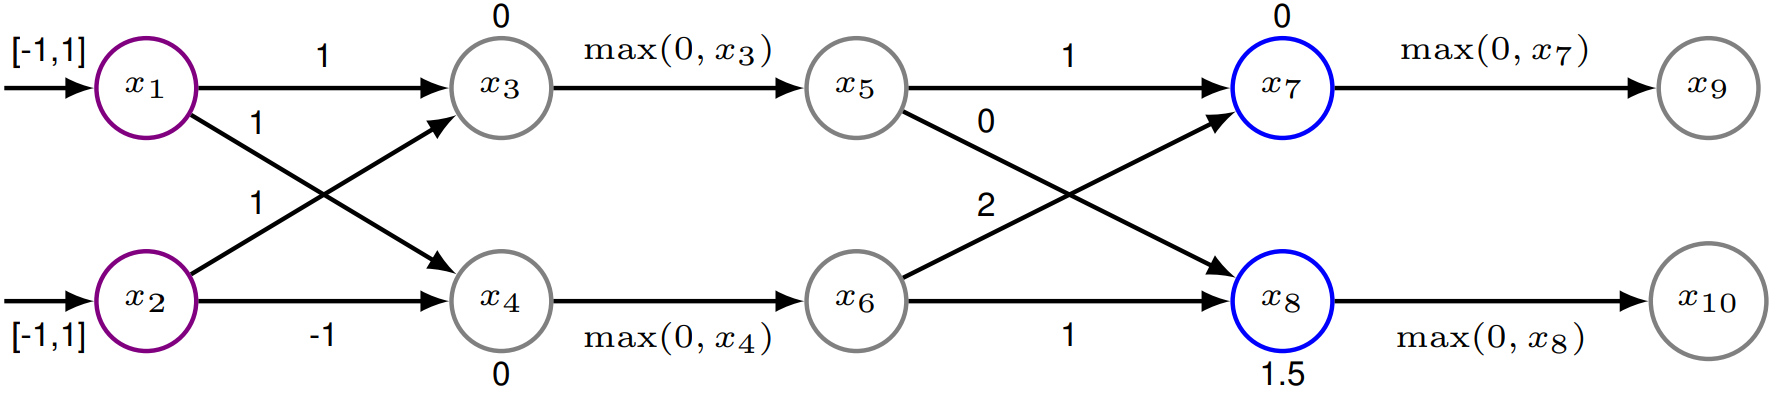
\includegraphics[scale=0.4]{example.png}
%	\caption{A DNN example from \cite{kneuron}, where every node is separated into its linear and its ReLU functions.}
%	\label{fig1}
%	\end{figure}
	
	\begin{figure}[t!]
		\centering
		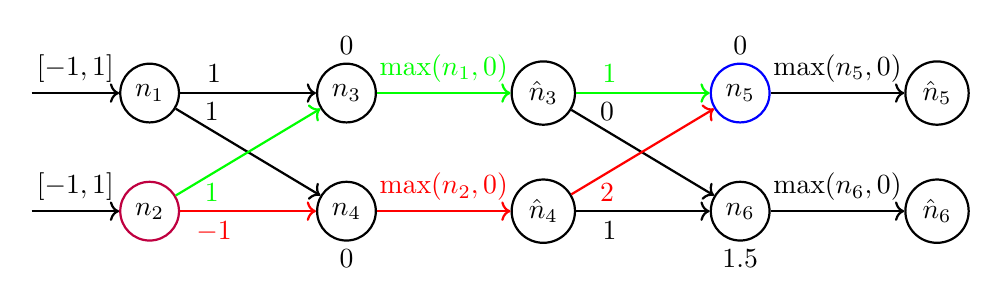
\begin{tikzpicture}
			
			\node[circle, draw= black, thick, minimum width = 20,
			minimum height = 20] (input1) {$n_1$};
			
			\node[circle, draw= purple, thick, minimum width = 20,
			minimum height = 20] (input2) at ($(input1) + (0,-1.5)$) {$n_2$};
			
			
			% Hidden layers
			
			\node (hidden10) at ($(input1) + (2.5,0.6)$) {$0$};
			
			\node (hidden20) at ($(input1) + (2.5,-1.5-0.6)$) {$0$};
		
			\node (hidden50) at ($(input1) + (7.5,0.6)$) {$0$};
			
			\node (hidden60) at ($(input1) + (7.5,-1.5-0.6)$) {$1.5$};
			
			
			\node[circle, draw= black, thick, minimum width = 20,
			minimum height = 20] (hidden1) at ($(input1) + (2.5,0)$) {$n_3$};
			\node[circle, draw= black, thick] (hidden2) at ($(input1) + (2.5,-1.5)$) {$n_4$};
			
			\node[circle, draw= black, thick, minimum width = 20,
			minimum height = 20] (hidden3) at ($(input1) + (5,0)$){$\hat{n}_3$};
			\node[circle, draw= black, thick] (hidden4) at ($(input1) + (5,-1.5)$) {$\hat{n}_4$};
			
			
			\node[circle, draw= blue, thick, minimum width = 20,
			minimum height = 20] (hidden5) at ($(input1) + (7.5,0)$){$n_5$};
			\node[circle, draw= black, thick] (hidden6) at ($(input1) + (7.5,-1.5)$) {$n_6$};
			
			
			
			
			% Output layer
			\node[circle, draw= black, thick, minimum width = 20,
			minimum height = 20] (output1) at ($(input1) + (10,0)$){$\hat{n}_5$};
			
			\node[circle, draw= black, thick, minimum width = 20,
			minimum height = 20] (output2) at ($(input1) + (10,-1.5)$){$\hat{n}_{6}$};
			
			
			% Connections
			
			\draw[->,thick] ($(input1) + (-1.5,0)$) -- (input1) node[midway, above] {$[-1,1]$};
			
			\draw[->,thick] ($(input1) + (-1.5,-1.5)$) -- (input2) node[midway, above] {$[-1,1]$};
			
			
			
			\draw[->,thick] (input1) -- (hidden1) node[near start, above] {$1$};
			\draw[->,thick] (input1) -- (hidden2)node[near start, above] {$1$};
			
			\draw[->,color=green, thick] (input2) -- (hidden1) node[near start, below] {$1$};
			\draw[->,color=red, thick] (input2) -- (hidden2)node[near start, below] {$-1$};
			
			
			
			
			
			\draw[->,color=green, thick] (hidden1) -- (hidden3) node[midway, above] {$\max(n_1,0)$};
			\draw[->,color=red, thick] (hidden2) -- (hidden4) node[midway, above] {$\max(n_2,0)$};
			
			
			
			
			
			\draw[->,color=green, thick] (hidden3) -- (hidden5) node[near start, above] {$1$};			
			\draw[->,thick] (hidden3) -- (hidden6) node[near start, above] {$0$};
			
			\draw[->,color=red, thick] (hidden4) -- (hidden5)node[near start, below] {$2$};
			\draw[->,thick] (hidden4) -- (hidden6)node[near start, below] {$1$};
			
			
			
			
			\draw[->,thick] (hidden5) -- (output1) node[midway, above] {$\max(n_5,0)$};
			\draw[->,thick] (hidden6) -- (output2) node[midway, above] {$\max(n_6,0)$};
			
			
		\end{tikzpicture}
		\caption{A DNN example from \cite{kpoly}: every neuron is separated into 2 nodes, $n$ pre- and $\hat{n}$ post-ReLU activation function. The pair $(n_2 n_3 n_5,n_2 n_4 n_5)$ in green and red is compensating (weights of paths are $1,-2$).}
		\label{fig1}
	\end{figure}
	
The idea to perform value abstraction is to compute upper and lower bounds on the values of (some) neurons in the DNN when the inputs are in a given neighbourhood, in order to conclude on the robustness without needing to compute the values exactly for all inputs (in the neighbourhood).

First, remark that weighted sums is a linear function, so it is easy to represent it explicitly. The only problematic part to represent accurately is the ReLU function. While it is fairly simple piecewise linear function with 2 modes ($x<0$ and $x \geq 0$), it is not linear. Considering its iterated impact along the different layers of a ReLU DNN is much more complex than it seems. First, let us remark that it is easy to represent exactly $\ReLU(x)$ in case $x$ is {\em stable}, that is, either it is known to be entirely positive, order
it is known to be entirely negative, as in both case there is only one known linear mode involved. Hence, the sole problem remains how to handle {\em unstable} neurons.

Consider the simpler abstraction, called the {\em Box abstraction} \cite{deeppoly}: inductively compute the bound on each neuron of the next layer independently, by considering the weighted sum over the bounds of the previous layer, then clip the lower bound at 
$\max(0,$ lower bound$)$ to represent the ReLU function, and so on.
For all $i$, let $x_i=\val_{\vx}(n_i)$, with $\vx=(x_1,x_2)$.
For instance, on the DNN example of Fig \ref{fig1}, $x_1,x_2 \in [-1,1]$, then $x_3,x_4 \in [-2,2]$, using ReLU $\hat{x}_3,\hat{x}_4 \in [0,2]$, and $x_5 \in [0,6]$ while $x_6 \in [0,2]$. 
While the bounds for $n_1, \ldots, n_4$ are exact (for all $\alpha$ 
in the range, there is an input $\vy$ such that $\val_{\vy}(n_i)=\alpha$), 
it is no more the case from the next layer (starting in $n_5,n_6$) because of potential 
dependencies between earlier neurons: $n_3$ reaches value $2$ only when $x_1=x_2=2$,
in which case $n_4$ reaches value $Val_{(2,2)}(n_4)=0$. Hence, it is impossible that $x_5=\Val_{\vx}(n_5)$ reaches $6$, as it would require both $n_3$ and $n_4$ to have value $2$.

A still extremely fast algorithm that corrects some of this issue is {\em DeepPoly} \cite{deeppoly}, also rediscovered as the {\em CROWN} algorithm \cite{crown}. Instead of 
hard bounds, for each neuron $n$ of layer $k$, two affine functions (with input at the previous layer $k-1$) are kept as lower bound and upper bound of the value of the node.
Denote $f_i \leq x_i \leq g_i$ with e.g.  
$f_{3}(x_3)=f_4(x_4)=0$ and 
$g_3(x_3) = \frac{x_3+2}{2}$,
$g_4(x_4) = \frac{x_4+2}{2}$. 
With that, we get 
$x_5 \leq g_3(x_3) + 2 g_4(x_4) = \frac{x_3 + 2x_4 + 6}{2} = \frac{3x_1 - x_2 + 6}{2}\leq 5$.

For $[\alpha,\beta]$ bounds on $x_i$, there is one optimal linear function for the upper bound $g_i(x_i)= \beta \frac{x_i-\alpha}{\beta-\alpha}$ for ReLU nodes.
There are two choices for the lower bound: $f^1_i(x_i) = 0$ or $f^2_i(x_i)=x_i$.
In the DeepPoly algorithm, the choice is made by considering $\alpha < 0 < \beta$ (for unstable neurons). If $|\alpha|\geq |\beta|$ then $f_i=f^1_i$ is used, while if $|\beta|>|\alpha|$ then $f_i=f^2_i$ is used. Denote {\em $\overline{\mbox{DeepPoly}}$} the DeepPoly algorithm such that $f^1_i$ is always used, and $f^2_i$ is never used. 
Unlike DeepPoly, {\em $\overline{\mbox{DeepPoly}}$} subsumes the {\em Box abstraction}. Indeed, taking bounds $[-0.2,5]$ on $x_i$, it gives $\ReLU(x_i) \in [0,5]$, 
while the normal DeepPoly algorithm would only allow to conclude that $\ReLU(x_i) \in [-0.2,5]$.

\iffalse
\subsection{PRIMA and $\beta$-CROWN}
\fi

\subsection{MILP and LP encodings for DNNs}

At the other end of the spectrum, we find the Mixed Integer Linear Programming (MILP) value abstraction, which is a priori a complete method (albeit much slower than DeepPoly). 
Consider an unstable neuron $n \in[\alpha,\beta]$. The value $x$ of $\ReLU(n)$ can be encoded exactly in an MILP formula with one integer (actually even binary) variable $a$ valued in ${0,1}$, using 4 constraints \cite{MILP}:
\vspace{-0.1cm}
\begin{align*}
	\hat{x} \geq x \quad \wedge \quad \hat{x} \geq 0, \quad \wedge \quad \hat{x} \leq \beta \cdot a \quad \wedge \quad \hat{x} \leq x-\alpha \cdot (1-a)
\end{align*}

From \cite{MILP}, for all $x \in [\alpha,\beta] \setminus 0$, there is a unique solution $(a,\hat{x})$ satisfying the constraints, and we have $\hat{x}=\ReLU(x)$ (and $a$ is 0 if $x < 0$ and 1 if $x>0$, and can be either for $x=0$). Such an encoding can be used for every (unstable) ReLU node, and optimizing its value allows to certify a given input. 
For Networks with hundreds of nodes or more, the associated MILP formula will have have hundreds of integer variables, and it will usually not be solvable efficiently.

MILP instances can be linearly relaxed into LP over-abstraction, where variables which were integers in $\{0,1\}$ (binary) are relaxed to be real in interval $[0,1]$, using otherwise the same encoding. Solving LP instances being Polynomial time, optimizing it is much more efficient, but at the price of a lack of accuracy (e.g. with not as tight bounds). This is called the {\em LP abstraction}.

As far as we know, no formal result states the relationship between the LP approximation and DeepPoly.
We prove now that the LP abstraction is strictly more accurate than the DeepPoly abstraction, as it actually corresponds to considering in DeepPoly both linear functions lower bounding the ReLU function, $ReLU(x) \geq 0$ and $ReLU(x) \geq x$, while DeepPoly considers exactly one.

\begin{proposition}
	\label{LP}
 Given $x \in [\alpha,\beta]$ with $\alpha < 0 < \beta$, the following two systems of constraints 
 1) for LP and 2) for DeepPoly with both lower bounds are equivalent:
 \vspace{-0.3cm}
 \begin{align*}
	 & 1) \quad \hat{x} \geq x \quad \wedge \quad \hat{x} \geq 0, \quad \wedge \quad \hat{x} \leq \beta \cdot a \quad \wedge \quad \hat{x} \leq x-\alpha \cdot (1-a), \, a \in [0,1] \\
	 \text{and} \quad  & 2)  \quad \hat{x} \geq x \quad \wedge \quad \hat{x} \geq 0 \quad \wedge \quad \hat{x} \leq \beta \frac{x-\alpha}{\beta-\alpha}
\end{align*} 
\end{proposition}

\begin{proof}
Obviously, the 2 lower bound constraints are the same in 1) and 2).

It remains to prove that the 2 upper bound constraints of 1) LP corresponds to the 2) DeepPoly linear upper bound. For that, we study the upper bound function in the linear variable $a \in  [0,1]$, with $x \in [\alpha,\beta]$ fixed. We have $\hat{x}$ in 1) is uppered bounded by $max_{a \in [0,1]} (min(\beta \cdot a, x - \alpha (1-a)))$, and this bound can be reached. 
The function $min(\beta \cdot a, x - \alpha (1-a))$ reaches its maximum for 
$\beta \cdot a = x - \alpha (1-a)$, that is 
$(\beta - \alpha) a = x - \alpha$, i.e. 
$$ a = \frac{x - \alpha}{\beta-\alpha}$$

It thus gives an upper bound at 
$\beta \cdot a = \beta \frac{x - \alpha}{\beta-\alpha}$, which is exactly the function used in DeepPoly.
\hfill $\square$
\end{proof}







\section{Compensating pairs of paths}
\label{Sec.comp}

In this section, we explore the key factor for the loss of accuracy in value abstraction methodologies, as those we presented before (except for full MILP which is exact but 
not efficient). 
Namely, we uncover that \emph{compensating pair of paths} are the reason for the loss of precision. A pair $(\pi,\pi')$ of paths is {\em compensating} if:
\begin{itemize}
 \item they have the same starting node $a$ (called {\em source} state) and ending node $b$ (called {\em target} state of $(\pi,\pi')$),
 \item they are disjoints (the only common nodes are the source and the target),
 \item the weights satisfy $weight(\pi') < 0 < weight(\pi)$.
\end{itemize}

For instance, on Fig.~\ref{fig1}, the paths $\pi= n_2 n_3 n_5$ has weight $1$, while the
path $\pi'= n_2 n_4 n_5$ has weight $-2$, hence $(\pi,\pi')$ is a compensating pair of paths.
We call a path $\pi$ {\em compensating} if there exists a path $\pi'$ such that either $(\pi,\pi')$ or $(\pi',\pi)$ is compensating.

Compensating pair of paths will make precision of the target state reduce when using overabstraction of values. Here, $x_5 \leq 4$, which is reached for $x_1=1$ and $x_2=-1$: 
$\val_{(1,-1)}(n_5)=4$. However, Box computes an upper bound of $6$, and while DeepPoly recovers some of the dependency in $x_2$, it can only cancel out some of $x_2$ value due to the ReLU over-abstraction (contribution of $\frac{-x_2+3}{2} \leq 2$ instead of exact $-x_2 \leq 1$), obtaining $x_5 \leq 5$ instead of the precise $x_5 \leq 4$.

Intuitively, the target state receives the weight from the source state from the different paths from the source to the target. As the weights of the paths is of opposite sign, some of these weights will cancel out, by an amount up to $min(|weight(\pi')|,|weight(\pi')|)$. 
Further, that also avoid accumulating the error, in the same way as $0= |1+(-1)| \leq |1|+|-1|=2$ from an inaccurate analysis. The amount of compensation can however be reduced by the ReLU functions, because of clipping by the ReLU function. For instance, consider that the inputs $x_1,x_2$ lies in $[-1,-0]$. Then $\hat{x}_3$ will always be 0 for any input $\vx=(x_1,x_2) \in [-1,-0] \times [-1,-0]$, and $weight(\pi')$ will not compensate $weight(\pi')$.




\iffalse
\vspace*{2ex}

\begin{figure}
\centering
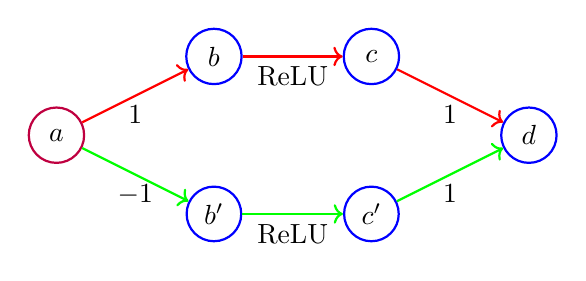
\begin{tikzpicture}
	
	\node[circle, draw= purple, thick, minimum width = 20,
	minimum height = 20] (input1) {$a$};

	
	% Hidden layers
	\node[circle, draw= blue, thick, minimum width = 20,
	minimum height = 20] (hidden1) at ($(input1) + (2,1)$) {$b$};
	\node[circle, draw= blue, thick] (hidden2) at ($(input1) + (2,-1)$) {$b'$};
	
	\node[circle, draw= blue, thick, minimum width = 20,
	minimum height = 20] (hidden3) at ($(input1) + (4,1)$){$c$};
	\node[circle, draw= blue, thick] (hidden4) at ($(input1) + (4,-1)$) {$c'$};
	
	% Output layer
	\node[circle, draw= blue, thick, minimum width = 20,
	minimum height = 20] (output) at ($(input1) + (6,0)$){$d$};
	
	% Connections
	\draw[->,thick,draw= red] (input1) -- (hidden1) node[midway, below] {$1$};
	\draw[->,thick,draw= green] (input1) -- (hidden2)node[midway, below] {$-1$};
	
	\draw[->,thick,draw= red] (hidden1) -- (hidden3) node[midway, below] {$\ReLU$};
	\draw[->,thick,draw= green] (hidden2) -- (hidden4) node[midway, below] {$\ReLU$};
	
	\draw[->,thick,draw= red] (hidden3) -- (output)node[midway, below] {$1$};
	\draw[->,thick,draw= green] (hidden4) -- (output)node[midway, below] {$1$};
\end{tikzpicture}
\end{figure}

\vspace*{2ex}

In this figure, $a$ is the input neuron; $bc,b'c'$ are nodes in the hidden layer, ($b,b'$ are pre-activation and $c,c'$ are post activation); and $d$ is the unique output neuron. The numbers next to the arrows are the weights. So, $W_{ba}=1$ and $W_{b'a}=-1$, $W_{dc}=W_{dc'}=1$. The pair of these two paths, $a$ to $bc$ to $d$, and $a$ to $b'c'$ to $d$, is a so called \emph{Compensating Pair}. Because its shape looks like a diamond, it is also called a Diamond. The characteristic is that, the products of all weights in the paths, have two different signs: along $bc$, the product is (strictly) positive, while along $b'c'$, the product is (strictly) negative. 

The existence of compensating pairs is key reason why simple approximation like LP or Interval Arithmetic cannot get the exact upper and lower bounds. If both pairs are negative or positive, LP or even Interval Arithmetic will get the exact values of lower and upper bounds.


To explain why, suppose we have another input node $a'$, such that both $a$ and $a'$ has an input interval $[0,1]$, but the weight from $a'$ to $b$ or $b'$ are both $1$. Then both $b$ will have an interval $[0,2]$ and $b'$ will have an interval $[-1,1]$. More importantly, in LP formulation, $c$ will be $b$ but $c'$ will be $0.5(b')+0.5$. The upper bound of $d$ will be $c+c'$, and hence $b+0.5(b')+0.5$, and hence $a+a'+0.5a'-0.5a'+0.5=0.5a+1.5a'+0.5$. And this will leads to a upper bound $2.5$ but this is not exact.

\vspace*{2ex}
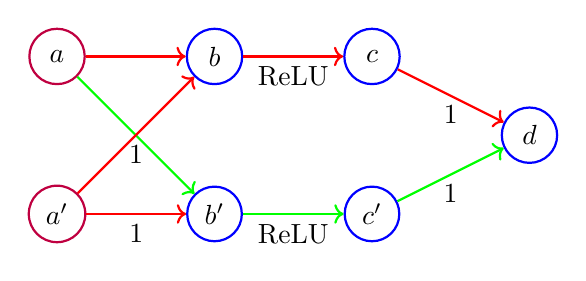
\begin{tikzpicture}
	\node[circle, draw= purple, thick, minimum width = 20,
	minimum height = 20] (input1) {$a$};
	
	\node[circle, draw= purple, thick, minimum width = 20,
	minimum height = 20] (input2) at ($(input1) + (0,-2)$) {$a'$};
	
	
	% Hidden layers
	\node[circle, draw= blue, thick, minimum width = 20,
	minimum height = 20] (hidden1) at ($(input1) + (2,0)$) {$b$};
	\node[circle, draw= blue, thick] (hidden2) at ($(input1) + (2,-2)$) {$b'$};
	
	\node[circle, draw= blue, thick, minimum width = 20,
	minimum height = 20] (hidden3) at ($(input1) + (4,0)$){$c$};
	\node[circle, draw= blue, thick] (hidden4) at ($(input1) + (4,-2)$) {$c'$};
	
	% Output layer
	\node[circle, draw= blue, thick, minimum width = 20,
	minimum height = 20] (output) at ($(input1) + (6,-1)$){$d$};
	
	% Connections
	\draw[->,thick,draw= red] (input1) -- (hidden1);
	\draw[->,thick,draw= green] (input1) -- (hidden2);
	
	\draw[->,thick,draw= red] (input2) -- (hidden1) node[midway, below] {$1$};
	\draw[->,thick,draw= red] (input2) -- (hidden2)node[midway, below] {$1$};
	
	\draw[->,thick,draw= red] (hidden1) -- (hidden3) node[midway, below] {$\ReLU$};
	\draw[->,thick,draw= green] (hidden2) -- (hidden4) node[midway, below] {$\ReLU$};
	
	\draw[->,thick,draw= red] (hidden3) -- (output)node[midway, below] {$1$};
	\draw[->,thick,draw= green] (hidden4) -- (output)node[midway, below] {$1$};
\end{tikzpicture}
\vspace*{2ex}

The general formal definition of compensating pair is as follows:

\begin{definition} In a full-connected network with $\ReLU$ as activation function:
	
	1. A path is a sequence of nodes $\langle a,b,c,d,e,\cdots\rangle$ of nodes that goes consecutively through each layer. We call the first node source node and the last node target node.  
	
	2. The \emph{Value} of a path is the product of of weights along the path (with sign): for a path $\langle a,b,c,d,e,\cdots\rangle$, its values is $$V = W_{ab}\cdot W_{bc}\cdot W_{cd}\cdot W_{ed}\cdot \cdots$$
	
	3. A \emph{Compensating Pair} is a pair of paths with the same source node and target node, such that the two paths have no common node, and the values of two paths have opposite signs (one is strictly positive and another is strictly negative).
	
	We also use \emph{Diamond} to call a compensating pair in the network.
\end{definition}

The following theorem shows the role of compensating pairs in the computation:

\fi

Hence, compensation is {\em one} factor of inaccuracy. We prove now that it is actually the {\em only} reason for inaccuracy, in the following meaning.
If there is no compensating path in the DNN, then any method/approximation at least as accurate as the Box abstraction, e.g. $\overline{\text{DeepPoly}}$ or LP, computes the exact upper and lower bounds for every node, that is:

\begin{table}[b!]
	\centering
	\begin{tabular}{|c|c|c|c|}
	\hline
		\text{Source/Target Layers}  &  \text{Natural DNN} & \text{Robust DNN} & \text{Ratio Natural vs Robust} \\ \hline \hline
	0 / 2 & 0.0304 & 0.00220  & 13.8x\\ \hline
	1 / 3  & 0.0313 & 0.00875 & 3.58x \\ \hline
	2 / 4  &  0.0267 & 0.00785 & 3.40x \\ \hline
	3 / 5  &  0.0253 & 0.00804  & 3.18x \\ \hline
\end{tabular}
\caption{Comparison of the average compensation strength over all the pairs of nodes of layer source/target between a DNN naturally-trained and a DNN robustly-trained using DiffAI \cite{DiffAI} with the same architecture and training set.}
\label{tab:compensation}
\end{table}


\begin{theorem}
	\label{th1}
	Let $n$ be any node of a DNN with {\em no} compensating path. For $[\alpha,\beta]$ the bounds computed by the {\em Box abstraction} for $n$, we have that for all $\gamma \in [\alpha,\beta]$, there exists an input $\vx$ such that $\val_{\vx}(n)=\gamma$.
\end{theorem}


The sketch of proof can be found in Section \ref{sec.proofs}. 
Notice that standard DeepPoly does not satisfies Theorem \ref{th1} (it does not necessarily refine Box), and therefore we are not sure PRIMA or $\beta$-CROWN that refine DeepPoly satisfies Theorem \ref{th1}, though it would be easy to fix by using $\overline{\text{DeepPoly}}$. Anyway, in practice, it is very unlikely to have a network without any compensating path, it is more of a theoretical results show in that compensation is the reason for inaccuracy.

This result has a first interesting application: explain why some DNNs are intrinsically easier to verify than others. This is the case for DNNs trained adversarially to be robust, vs same architecture, but trained in a "natural" way \cite{deeppoly,prima,crown}. Indeed, compensating pairs is a purely structural property on the DNN learnt, rather than more semantical notions, such as the number of unstable ReLUs, which depends heavily upon the image considered and the algorithm used. We compare compensations with source and target separated by 1 ReLU layer, e.g. source in layer 0 and target in layer 2, for two Networks with 5 hidden layers of 100 nodes each from the ERAN GitHub repository, one trained naturally ("$6\times100$"), 
and one trained using DiffAI \cite{DiffAI} ("$5\times100$"). 
We report in Table \ref{tab:compensation} the average compensation strength, i.e. 
the average of $max_{\pi,\pi'} min(|weight(\pi')|,|weight(\pi')|)$
over all source/target states in given layers. The average compensations strength are much lower in the Robust DNN than in the natural DNN, and indeed the Robust DNN is much simpler to verify than the natural DNN (e.g. DeepPoly is more accurate and verifies more images).


\subsection{MILP$_{X_n}$}

While Theorem \ref{th1} is interesting to understand that compensation is a key notion for accurate verification of DNNs, it cannot be used directly to analyze DNNs with compensations, which are actually those that are most interesting to tackle.
Intuitively, when there are compensating paths, it seems necessary to consider exactly the (unstable) ReLU nodes that are seen along these paths. 
Consider a neuron $n$ in layer $k$ for which we want to have accurate bounds 
$[\alpha,\beta]$.
Let $X_n$ be the set of neurons $x$ in layer up to $k-1$ such that there is a compensating path with target $n$ passing by $x$ (but not as its source or target). Let $Y_n$ be the complement of this set $X_n$ of neurons in the first $k-1$ layers. We denote by MILP$_{X_n}$ the relaxation of the MILP encoding where all the nodes in $Y_n$ are linearly relaxed (thus with $|X_n|$ binary variable, one per neuron in $X_n$), and including exact bounds for every neurons $n'$ in the first $k-1$ layers. We state now that the bounds $[\alpha,\beta]$ on neuron $n$ computed by such MILP$_{X_n}$ are accurate.

\begin{theorem}
	\label{th2} 
	Let $n$ be any node of a DNN. Then for $[\alpha,\beta]$ the bounds computed by MILP$_{X_n}$ for neuron $n$, for all $\gamma \in [\alpha,\beta]$, there exists an input $\vy$ such that $\val_{\vy}(n)=\gamma$.
\end{theorem}

The sketch of proof of Theorem \ref{th2} can be found in Section \ref{sec.proofs}.


\subsection{Sketch of Proofs}
\label{sec.proofs}

%Intuitively, our first proof shows that if there are no compensation, then there are no correlations between nodes.
Consider a target neuron $z$.
In case there is no compensating path, we can assign a sign to each neuron $n$: 0
if all paths from $n$ to $z$ has weight 0, $+1$ if all paths have positive weights, and 
$-1$ if they have negative weights. Then we prove:

\begin{proposition}
	\label{prop.sign}
There exist two inputs $\vx^\star,\vx^\sharp$ such that ${\vx^\star}$ maximizes the value of all positive neurons and minimizes the value of all negative neurons, and  ${\vx^\sharp}$ minimizes the value of all positive neurons and maximizes the value of all negative neurons.
\end{proposition}

Hence $\val_{\vx^\star}(z)=\beta$ and $\val_{\vx^\sharp}(z)=\alpha$,
for $[\alpha, \beta]$ the bounds computed by the Box abstraction. We conclude Theorem \ref{th1} by invocking continuity.

\smallskip

Concerning Theorem \ref{th2}, consider an output node $z$.
Let $[\alpha(z),\beta(z)]$ be the bound computed by $\MILP_{X_z}$.
%We will show the existence of $\vx^\sharp,\vx^\star$
%such that $\val_{\vx^\sharp}(z)=\alpha$ and $\val_{\vx^\star}(z)=\beta$,
%and we will get the proof of Theorem 2 by a continuity argument.
%For that, 
We partition the input neurons from layer $0$ into:
\begin{enumerate}
	\item $A_{zero}= \{a \mid \forall \text{ path $\pi$ from $n$ to } z, weight(\pi)=0\}$.
	\item $A_{pos}= \{a \mid \forall \text{ path $\pi$ from $n$ to } z, weight(\pi)\geq0\}$.
	\item  $A_{neg}= \{a \mid \forall \text{ path $\pi$ from $n$ to } z, weight(\pi)\leq0\}$.
	Let $A_{pure}=A_{pos} \cup A_{neg}$.
	\item $A_{open}$ is the set of remaining input neurons.
\end{enumerate}

We then partition the set of neurons in hidden layers: 
\begin{enumerate}
	\item $B_{zero}= \{n \mid \forall \text{ path $\pi$ from $n$ to } z, weight(\pi)=0\}$.
	\item $B_{open}$ is the set of neurones reachable from $A_{open}$ and such that there is at least one path to $z$ with non zero weight.
	\item $B_{pure}$ is the set of remaining neurons.
\end{enumerate}

We can define the sign function for neurons in $A_{pure}$ and $B_{pure}$.
Further, the value of any neuron $n$ in $A_{pure}$ or $B_{pure}$ is entirely determined by 
nodes in $A_{pure}$ or $B_{pure}$. Therefore, applying Prop. \ref{prop.sign} on the DNN
made of nodes from $A_{pure}$ and $B_{pure}$, we obtain 
$\vx_{pure}^\star,\vx_{pure}^\sharp$ optimizing neurons in $A_{pure}$ or $B_{pure}$.
We can prove that there exists input 
$\vx^\star$ extending $\vx_{pure}^\star$
and input $\vx_{pure}^\sharp$ extending $\vx_{pure}^\sharp$
from $A_{pure}$ to $A_{pure} \cup A_{open}$ such that 
$\val_{\vx^\star}(z)=\beta(z)$ and $\val_{\vx^\sharp}(z)=\alpha(z)$.

The formal proofs are in appendix.


\subsection{An efficient algorithm}

Using Theorem \ref{th2}, one could thus obtain accurate bounds by running MILP$_{X}$ inductively on every node layer by layer, obtaining accurate bounds $[\alpha,\beta]$ that can be used to compute the next layer accurate bound. In practice, such an algorithm would however be inefficient, as $X_n$ comprises most of the nodes from layer up to $k-1$ for $n$ on layer $k$. Instead, an interesting trade off between speed and accuracy is to set a threshold on the the strength of compensation that are meaningful, and consider that paths below this threshold are not compensating strongly enough to deserve an integer variable, calling $Z_n$ the resulting set of nodes on {\em strongly compensating} paths. In practice, one could take the $K$ nodes covering the strongest compensating pair of paths to obtain set $Z_n$, for $K$ reasonably small. The pseudo-code of the algorithm is provided in Algorithm \ref{algo1}.

\SetKwInput{KwInput}{Input}
\SetKwInput{KwOutput}{Output}
	
\begin{algorithm}[b!]
	\caption{Compensate(K)}
	\label{algo1}
	\KwInput{Bounds $[\alpha_n,\beta_n]$ for input nodes $n$ at layer $0$ (input neighbourhood)}
	
	\KwOutput{Bounds $[\alpha_n,\beta_n]$ for every node $n$}
	 
	 \For{layer $k=1 \cdots \ell$}{
		\For{neuron $n$ in layer $k$}{
	
	 		Compute $Z$ a set of $K$ nodes covering the compensating pairs of paths with target $n$
			with heaviest compensation
		
			Run MILP$_Z$ to obtain $[\alpha_n,\beta_n]$ from bounds of neurons in layers $< k$
	 }
	 }
	 \end{algorithm}	
	
	
	

This algorithm has a worst case complexity bounded by $O(N \MILP(N,K))$, 
where $N$ is the number of nodes of the DNN, 
and $\MILP(N,K)$ is the complexity of solving a MILP program with $K$ integer variables and $N$ linear variables.
We have $\MILP(N,K) \leq 2^K \LP(N)$ where $\LP(N)$ is the Polynomial time to solve a Linear Program with $N$ variables.
This complexity is an upper bound, as e.g. Gurobi is fairly efficient and never need to consider all of the $2^K$ ReLU configurations to compute the bounds.
Notice that the for loop on neurons $n$ in layer $k$ at line 2 can be realized in parallel as we only need bounds from previous layers, not from the current layer $k$, 
leading to a time complexity of $O(\sum_{i=1}^{\ell} \MILP(N_{i-1},K))$, with $\ell$ the number of layers and $N_i$ the number of neurons in layers $0, \ldots, i$.
Hence, for $K$ small enough, Algorithm \ref{algo1} calls many times MILP (e.g. Gurobi)
with a limited number of integer variables, which should be efficient enough, and yet be quite accurate as it can compute exactly (Theorem \ref{th2}) the highest compensating path, which we verify in the next section.





\iffalse
\section{Verification Framework}



%Our experiments are carried by different version codes, and the global process has been changed. 

In this section, we will sketch the framework. 

\subsection{Structure}

\subsubsection*{Precomputation}

The open node chosen is the key part of the whole framework but costs a lot of time. So some computation (those do not rely on certain image and bounds) is moved to the precomputation part.

%The precomputation corresponds to the simplest case: source node fixed. We will compute and store a limited number of paths with highest (absolute) values before running any image. This does not rely on other parameters or results(bounds).
%
%Before build an MILP model and when choosing open nodes list,  the program will read the reference data combining with the data of bounds to continue the computation of open nodes. This will use much less time.



\subsubsection*{Process for one image} An image is the basic unit in whole process. The process of one image is simple: compute the concrete bounds of nodes layer by layer, use the bounds of previous layer to build MILP models of current layer. In one layer, nodes runs in parallel.

%Suppose we have reached a new layer $l_i$ and have upper and lower bounds of all nodes in previous layers. Then we will compute bounds of every node in $l_i$ in parallel using the data of bounds of previous nodes. The method is to build and optimize an MILP model.

%Some parameters may be changed during layers. Among all parameters, two groups are the most important: numbers of open nodes and local timeout parameters. Here, \emph{local} is opposite to \emph{global}. We have global timeout parameters for images and the whole running. Local timeout are used in one layer, one node, one model, or one loop in the optimization for a model.




%The open node chosen is the key part of the whole framework, and it will cost two much time without precomputation because we must do open node chosen for every node. 
%
%The precomputation corresponds to the simplest case: source node fixed. We will compute and store a limited number of paths with highest (absolute) values before running any image. This does not rely on other parameters or results(bounds).
%
%Before build an MILP model and when choosing open nodes list,  the program will read the reference data combining with the data of bounds to continue the computation of open nodes. This will use much less time.

\begin{algorithm}
	\caption{The Frame work}
	\KwData{Input Domain: $\mathcal{D}$}
	\KwResult{Bounds of all nodes: $\mathcal{B}$}
	
	Constant $\mathcal{R}$  \tcp*{Stored precomputation data}
	
	Constant $\boldsymbol{W}, \vb$ \tcp*{Weights and Bias of network}
	
	Constant Layers = $[0,1,2\cdots,L]$ \tcp*{lists of all layer}
	
	Constant NodesLayer = $[Nodes_0,Nodes_1,\cdots, Nodes_L]$ \tcp*{list of nodes in each layer}
	
	
	Initialize $\mathcal{B}$ = \{\} \tcp*{To store upper and lower bounds of all nodes}
	
	\For{$l$ in Layers}{
		\If{$l$ = 0}{
			
			$\mathcal{D}$, $\boldsymbol{W}, \vb$ $\rightarrow$ $\mathcal{B}_0$ = \{$x$: $(UB(x),LB(x))$,$\cdots$\} 
			\tcp*{Do linear transformation  from input to the first layer}
			
			Add \{$x$: $(UB(x),LB(x))$,$\cdots$\} to $\mathcal{B}$} 
		
		\Else{
			
			$l$, NodesLayer $\rightarrow$ $Nodes_l$ = $[x_0,x_1,\cdots]$
			
			\For{$x$ in $Nodes_l$}{
				$x$, $\mathcal{B}$, $\mathcal{R}$  $\rightarrow$ $\mathcal{O}$ \tcp*{To get the open node list $\mathcal{O}$}
				
				$\mathcal{B}$, $\boldsymbol{W}, \vb$, $\mathcal{O}$ $\rightarrow \mathcal{M}$  \tcp*{MILP model $\mathcal{M}$ for node $x$}
				
				\While{}{$\mathcal{M}$ $\rightarrow UB(x),LB(x)$ \tcp*{Optimization}}
				
				Add \{$x$: $(UB(x),LB(x))$\} to $\mathcal{B}$
				
				
			}
			
		}
		
		
	}
	
	\Return{$\mathcal{B}$}
	
\end{algorithm}

\subsubsection*{Process for one node}

 The optimization of a model consists of loops. For each loop, the model will do optimization by a timeout and observe the result. If it gets improvement, then continue the loop until the optimize bounds or the longer timeout. Otherwise it will give up optimization and store the best bounds obtained so far.  



\subsubsection*{Global Process}

In the newest version, we do images by batches for 100 images each. For each batch, the running consists of three turns, very fast turn, fast turn and slow turn.

In the very fast turn, it will run DeepPoly for all images to get a preliminary bounds for all nodes and verify the easiest images. Images verified and images with false predication will be deleted from the image list.

Then sort all remain images by the size of uncertainty of DeepPoly from smaller to larger. The fast turn is to run the images from the smaller side to larger side until consecutive two images cannot be verified. All remain images and images tried but not verified will be put into the next list. And then run the list with parameters for slow turn.




\subsection{Parameters}

Parameters like open node parameter $O$ is important in the frame. Basically, all parameters will be reset after one image.

\subsubsection*{Global parameters}




\subsubsection*{Local parameters}

$O$ and timeout parameters for loops will change frequently during the loops of one node. These change will not reset until the end of one layer or one image.



\subsection{Other Setting}

In our experiments, we have not used PGD-attack to exclude some images. In principle, there is no obstacle to use PGD-attack.
\fi














\section{Experimental Evaluation}

Our experimental evaluations have 3 goals:
\begin{enumerate}
  \item Evaluate experimentally how the choice of the set $Z$ impacts the accuracy of $\MILP_Z$, and compare different choices for $K$ the size of $Z$,
  \item Evaluate on benchmarks the percentage of certification that can be obtained
 using the compensation idea, and compare with competing efficient tools,
  \item Evaluate how the runtime of compensate($K$) scale with the size of DNNs.
\end{enumerate}

\subsection{Setting}
The benchmarks were run on an AMD 5975WX ($32$ cores$@3.6$GHz, 7nm, year 2022) with 256 GB of main memory and 2 NVIDIA RTX 3090. Gurobi 9.52 was used for solving MILP and LP problems. Our implementations for Compensate($K$) is entirely realized in Python 
$3.8.10$, and therefore not particularly optimal.

The local robustness verification is performed on DNNs trained for the MNIST image dataset as its the only DNNs naturally trained ("MLP" (fully connected Multi Level Perceptron) $5\times 100$, $5\times 200$, $8 \times 100$, $8 \times 200$) benchmarked by \cite{crown} not using robust training, and they are the hardest DNNs to verify, despite their relatively limited size (600 to 1600 neurons in hidden layers). Indeed, today's efficient methods leave between $12\%$ to $20\%$ of the images neither certified robust \cite{crown} nor with an attack to robustness found \cite{attack}, making them interesting DNNs to consider when improving accuracy. MNIST contains grayscale images of size $28 \times 28$ pixels ($752$ input neurons). For our evaluation, we evaluate on the standard first 1000 images of the dataset, to be directly comparable to experiments run in other papers, e.g. \cite{prima,crown}. We also experimented on (MLP) $6\times 500$ (results not reported in \cite{prima,crown}), checking the first 200 images of the dataset, as it takes a long time to run. Each DNN is associated with a $\varepsilon>0$ for the $L^\infty$ norm.
%, and a target label for verification. 


\subsection{Choosing nodes based on Compensation strength}

The first group of experiments we run, tests the accuracy of choosing a set $Z$ of $K$ nodes using compensation strength, compared with randomly choosing the same number $K$ of nodes (similar to MIPplanet \cite{MIPplanet}),  to understand if the choice is meaningful or any set $Z$ with the same size will result in a similar accuracy.

To measure the accuracy, we measure the uncertainty of all nodes in a layer:
the uncertainty of a node is the range between its computed lower and upper bound. 
We then average the uncertainty among all the nodes of the layer.
Formally, for a node $n$ with bounds $[\alpha,\beta]$, its uncertainty $unc(a) = \beta - \alpha$, and the average uncertainty of a layer $l$ is $\dfrac{\sum_{a\in l} unc(a)}{|l|}.$

We experiment with the smallest network (MLP $5\times 100$ in \cite{crown}, 
$5 \times 100$ in \cite{prima}, and abusively called $6 \times 100$ in \cite{deeppoly}), so that we can obtain exact bounds for the first few layers using a full MILP encoding of the DNN. We test over the $\vx=59$th image in the MNIST dataset, as it has a large number of unstable ReLU nodes in the first few layers ($61$ in the first and $55$ in the second layer), so we can experiment with a larger choice of values) for $K$.

\subsubsection*{ReLU Node in the first hidden layer}


\begin{table}[b!]
	\centering
	\begin{tabular}{|c||c|c|}
	\hline
	\text{Number $K$ of nodes in $Z$}  &  \text{Compensate strength} & \text{Random Choice}  \\ \hline
	\hline
	0  &  2.22 & 2.22  \\ \hline
	10  &  1.84 & 2.03  \\ \hline
	20  &  1.50 & 1.82  \\ \hline
	30  &  1.28 & 1.62  \\ \hline
	40  &  1.14 & 1.44  \\ \hline
	50  &  1.06 & 1.23  \\ \hline
	61 (max) & 1.05 &  1.05 \\ \hline
\end{tabular}
\caption{Average uncertainty of $\MILP_Z$ for nodes of the second layer, for $Z$ with $K$ ReLU nodes of the first layer (compensating strength vs random choice).}
\label{tab:example0}
%\vspace{-0.8cm}
\end{table}


We first experiment with the choice of nodes in the first hidden layer, and its consequences on the accuracy of nodes in the second layer.  Let $c$ be a node of the second layer.
A compensating pair $(\pi,\pi')$ of paths with target $c$ is thus of the form a node $a b c$ and $a b' c$, with $a$ an input node and $b,b'$ on the first layer. The compensating strength for $(b,b')$ is defined as $comp(b,b')=\sum_a \val_{\vx}(a) \min(weight(abc),weight(ab'c))$. Indeed, the pair $(a b c,a b' c)$ of path cannot compensate more than $\val_{\vx}(a) \min(weight(a,b,c),$\newline $weight(a,b',c))$, and $b,b'$ would help compensated the set of pairs of paths $\{(a b c,a b' c) \mid a$ is in the first layer$\}$. After selecting the heaviest $(b_0,b_0')$, we can then compute $comp(b)= \sum_{b' \text{already selected}} comp(b,b')+comp(b',b)$ and select iteratively the heaviest $b$'s one by one till reaching the threshold. 
%We do this for all node $c$ of the second layer.

We report in Table \ref{tab:example0} the average uncertainty of $\MILP_Z$ following the choice of the $K$ heaviest compensating ReLU nodes in $Z$, vs choosing $K$ nodes randomly. The range of uncertainty created by inacurate computations is up to $1.17=2.22-1.05$, $2.22$ being the accuracy provided by LP, and $1.05$ by an exact MILP encoding of all the unstable ReLU nodes. Selecting $30$ out of the $61$ unstable ReLU nodes, the uncertainty created by inacurracy is reduced by $80\%$, while a random choice of nodes only leads up to roughly halving this number. We can deduce that selecting nodes based on compensating strength helps to select important ReLU nodes for the accuracy.



\newpage 

\subsubsection*{ReLU Node in the first and second hidden layer}

We now turn to evaluating choosing ReLU nodes in two consecutive layers, focusing on the uncertainty of nodes in the third layers, wrt ReLU nodes in the first and second layer.
The bounds for nodes of the first two layers are computed exactly. 
Let $d$ be a neuron of the third layer.
We keep the previous evaluation for ranking nodes in the previous (second) layer. 
Once the set $Z$ of selected nodes has sufficiently many nodes $c,c'$ in the second layer, adding $b,b'$ from the first layer to $Z$ allows to take into account accurately the pairs of paths of the form $(a b c d, a b' c' d)$ for all $\{c,c'\} \in Z$. We thus define:
\vspace{-0.2cm}
$$comp(b,b')=\sum_a \sum_{c,c' \in Z} \val_{\vx}(a) \min( weight(abcd),weight(ab'c'd))$$ 
\vspace{-0.2cm}

and the associated $comp(b)$, and select iteratively nodes $b$ (first layer) or $c$ (second layer) by selecting the heaviest $comp(b)$ or $comp(c)$.

We report in Table \ref{tab:example1} the average uncertainty of $\MILP_Z$ following the choice of the $K$ heaviest compensating ReLU nodes in $Z$, vs choosing $K$ nodes randomly from layers $1$ and $2$. 
We compare choosing nodes in the second layer only with choosing nodes in both the first and second layer.
Choosing ReLU nodes in the previous layer (layer $2$) only is less accurate than 
also choosing nodes in layer $1$. When picking in both layer $1$ and $2$, choosing $50$ out of $116$ unstable ReLU nodes allows to reduce by $90\%$ the average uncertainty due to inaccurate computations ($0.059$ vs $0.574$), while it only reduces the inaccuracy by $65\%$ when choosing nodes randomly. Notice that applying this layer after layer will even further reduce uncertainty created by accumulation of inaccuracies. Last, it is likely that selecting ReLU nodes in 1,2,3 layers earlier (for nodes in layer $4+$) could further improve the accuracy, but the computational trade-off to evaluate the compensating strenght of such paths is unclear and we thus did not experiment. 

\begin{table}[t!]	
	\centering
	\begin{tabular}{|c||c|c|c|}
	\hline
	\text{Number $K$}  &  \text{Compensate layer} 1+2 &  \text{Compensate layer} 2 & \text{Random layer } 1+2 \\ \hline
	\hline
	0  &  1.758 & 1.758 & 1.758  \\ \hline
	10  &  1.677 & 1.677 & 1.695  \\ \hline
	20  &  1.539 & 1.567 & 1.622  \\ \hline
	30  &  1.431 & 1.489 & 1.542  \\ \hline
	40  &  1.329 & 1.454 & 1.47  \\ \hline
	50  &  1.243 & 1.432 & 1.39  \\ \hline
	116 &  1.184 & 1.422 & 1.184  \\ \hline
\end{tabular}
\caption{Average uncertainty of $\MILP_Z$ for nodes of the third layer, for $Z$ with $K$ ReLU nodes of the 1st and 2nd layer (compensating strength vs random choice).}
\label{tab:example1}
%\vspace{-0.8cm}
\end{table}

\subsection{Comparison to efficient Verifiers}


In terms of efficient verifiers we compare with, we report:
\begin{itemize}
	\item DeepPoly \cite{deeppoly}/ CROWN \cite{crown}. We report the runtime from our own implementation used in Compensate($K$). It shows that our purely Python implementation is not optimal ($10$-$100$ times slower than the implementation in ($\alpha$)($\beta$)CROWN, ERAN and PRIMA). Our aim is indeed not to have the most optimized tool, but to evaluate the accuracy of Compensation.
	\item PRIMA, with results reported in \cite{prima} and \cite{crown}, as it is the closest in practice with our algorithm, computing accurate bounds for all neurons (as we do), although with a different technique: they focus on explicit correlations between neurons, while we consider the correlations indirectly through a better network abstraction. They use GPU while we do not. When computing the whole correlated space, 
	parallelization is difficult.
	Notice that on these MLP networks, PRIMA resort to refined bounds on the first few layers (3 or 4) using exact MILP encoding of all the nodes (which is easily parallelized - 16 nodes considered in parallel in PRIMA). This is doable on the first few layers as the number of integer variable is not too large. By comparison, we run MILP on all the layers, but with a bounded number of integer variables to control the runtime and to scale to all the layers.
	\item ($\alpha$)$\beta$-CROWN, with results as reported in \cite{crown}, as it is the most accurate of the efficient tool to date. Its main idea is to implement a very efficient Branch and Bound (BaB) verification tool, subsuming \cite{BaB}, and heavily using GPU implementation (while we do not). Performance of pure BaB on these hard DNNs is however impaired by the large number of branchs to consider. Similarly as PRIMA, $\beta$-CROWN resorts to refining the bounds of the first few layers using an exact MILP encoding, also computing 16 nodes in parallel, before running their BaB tool. 
	\item We also experimented with the latest versions of $\alpha$-$\beta$-CROWN (October 2023) and PRIMA (2022) on MLP $6 \times 500$ (results not reported in \cite{crown,prima}).
	\item We do not report results from kPoly \cite{kpoly}, OptC2V \cite{optC2V}, 
	SDPFO \cite{SDPFI}, MIPplanet \cite{MIPplanet} which do not present favorable trade offs compared with $\beta$-CROWN. Results can be found in \cite{crown} and are performed in the same conditions so can be compared.
	\item Finally, we run several version of Compensate($K$) ({\color{blue} Comp} in Table \ref{tab:example}). First, we have a fixed choice for $K$ ($K=60$ for fast and $K=200$ for slow), with a fall back to a lower $K$ ($K=50$ for fast and $K=60$ for slow) if the bounds found is too far from the solution found (MIPGap $>0.5$ in Gurobi). We run (our implementation of) DeepPoly first, then the fast version, before running slow on the remaining images.
	Further, we also experiment with an {\em adaptative} implementation, which lowers number $K$ adaptively between layers to adapt to the growing number $N$ of linear variables, which has an impact on the overall $\MILP(N,K)$ runtime. This is particularly useful for deeper network where $N$ is very different between the first and the last layer. Again, we run first an aggressive version of fast, before going to a more conservative slow version to treat the remaining images. All versions compute bounds for 20 neurons of the same layer in parallel, no GPU used.
\end{itemize}


In Table \ref{tab:example}, we report the accuracy and runtime of these different methods.
DeepPoly/CROWN is by far the fastest, but also the most inaccurate, certifying robustness for less than $30\%$ of the images, whereas there are at least $82\%$ of the images for which no attacked is found (attacks computed by \cite{attack} in $\beta$-CROWN).
This is because these DNNs, although of reasonable size, are hard to verify (they are trained in a natural way, with high compensation strength, see Section \ref{Sec.comp}).


Compared with PRIMA (using refinement of the first few layers by exact MILP), the overall method is quite similar, looking at all the nodes one by one from the beginning of the network till the end. Our method compare favorably, both in terms of time and accuracy: our fastest setting is always faster than PRIMA, sometimes by a large margin ($>3$ times faster on $8 \times 100$ while verifying $10\%$ more images), and also more accurate (except our fast adaptative method for $5 \times 200$ which is quite pointless on this shallow DNN - the fixed method is both faster and more accurate than PRIMA), sometimes by a large margin (by $14 \%$  for $5 \times 100$ while being $30\%$ faster). Further, unlike PRIMA, we do not resort to a GPU, and our purely Python implementation is not optimal. This is very promising for this idea of compensation, which indirectly treats dependencies between the variables, which PRIMA represents explicitly.



\begin{table}[t!]
	\centering
	\begin{tabular}{|c||c|c|c||cc|cc||c|}
		
		\hline
		\text{DNN}  & DeepPoly & PRIMA & $\beta$-CROWN &\multicolumn{2}{@{}c@{}|}{\color{blue}\text{ Comp (adapt.) }} & \multicolumn{2}{@{}c@{}|}{\color{blue} \text{ Comp (fixed) }} & Upper\\ 
		 & / CROWN & (refined) & (refined BaB) & {\color{blue}fast} & {\color{blue}slow} & {\color{blue}fast} &{\color{blue}slow} & Bound\\
		\hline \hline
		
		$5 \times100$\  &   $16\%$ & $51\%$ & $\mathbf{69.9\%}$ & {\color{blue}$57.5\%$} & {\color{blue}$66.1\%$} & {\color{blue}$65.3\%$} & {\color{blue}$68.4\%$} &  $84.2 \%$ \\ 
		$\epsilon = 0.026$ & 5s & 159s & 102s& {\color{blue}75s} & {\color{blue}140s} & {\color{blue}117s} & {\color{blue}142s} &  \\
		\hline	
		
		$5 \times 200$ \  &  $18.2\%$ & $69\%$ & $\mathbf{77.4\%}$ & {\color{blue}$64.3\%$} & {\color{blue}$74.7\%$} & {\color{blue}$72\%$} & {\color{blue}$76.8\%$} & 
		$90.1 \%$\\ 
		$\epsilon = 0.015$ & 11s & 224s & 86s & {\color{blue}163s} & {\color{blue}285s} & {\color{blue}206s} & {\color{blue}279s}  &\\ \hline \hline

	
		$8\times100$\  &   $29.2\%$ & $42.8\%$ & $62\%$ & {\color{blue}$52.7\%$} & {\color{blue}$59.7\%$} & {\color{blue}$61.4\%$} & {\color{blue}$\mathbf{65.8\%}$}  & $82.0 \%$ \\ 
		$\epsilon = 0.026$ & 8s & 301s & 103s & {\color{blue}92.3s} & {\color{blue}179s} & {\color{blue}170s} & {\color{blue}346s} & \\
		\hline
	

		$8\times200$\  &   $25.9\%$ & $62.4\%$ & $73.5\%$ & {\color{blue}$68.1\%$} & 
		{\color{blue}$\mathbf{79.1\%}$} & {\color{blue}$72.6\%$} & {\color{blue}too} & $91.1 \%$ \\ 
		$\epsilon = 0.015$ & 17s & 395s & 95s  & {\color{blue}297s} & {\color{blue}535s} & {\color{blue}$480s$} & {\color{blue}slow} & \\ \hline
		
		%6$\times$500\  &   0.035& 1.758 & time & 1.758 & time &    1.758 & time & 1.758 & time & \\ 
		%$\epsilon = 0.035$ & & & & & & & & & &\\ \hline
	\end{tabular}
	\caption{$\%$ of verified images and average runtime in seconds, over 1000 images. 
	Results for PRIMA, $\beta$-Crown and the upper bound on the $\%$ are from \cite{crown}.}
	\label{tab:example}
	\vspace{-0.8cm}
\end{table}


Compared with $\beta$-CROWN (also using a refinement on the first few layers using exact MILP), 
the picture is more balanced, because the fundamentals of both algorithms are different. BaB 
focuses on the output neuron, computing bounds for it, and refining the different ReLU as necessary. 
Instead, we consider every node one by one from the input layer till the final layer, with the same accuracy. Hence our algorithm will spend a lot of time on nodes which are not necessary for the verification. Therefore, our naive implementation is not as efficient as the highly optimized
$\beta$-CROWN: our implementation is 2 to 5 times slower than $\beta$-CROWN, while we are not using GPU, unlike $\beta$-CROWN. Things are more interesting on the accuracy front: on shallower DNNs ($5 \times 100$ and $5 \times 100$ with 5 hidden layers), the refinement with MILP treats all but the 2 last layers, 
leaving BaB with few ReLU nodes to branch on, and $\beta$-CROWN (refined BaB) is slightly more accurate than using compensation: we are within $1.6\%$ of the accuracy. On deeper DNNs ($8 \times 100$ and $8 \times 100$ with 8 hidden layers), the refinement with MILP cannot treat the 4 last layers, and BaB has more ReLU to branch on. Therefore, Compensate($K$) is more accurate than $\beta$-CROWN, 
closing the gap with the upper bound from $20\%$ to $16.2\%$ ($8 \times 100$)
and from $17.6\%$ to $12\%$ ($8 \times 200$). This is very promising for the compensation idea, which could be used in many different ways than Compensate($K$) (see next Section).
 

\newpage

Importantly, ($\alpha$)$\beta$-Crown, while efficient, can face a (complexity) wall, when the number of branches becomes too extreme for BaB to work: either BaB succeds fast, or it will not suceed even with very long time out (the reason why {\em refined} BaB is more accurate on these networks). We verify that in Table \ref{tab:example3}, on a larger DNN learnt in a natural way, namely MLP $6 \times 500$,.
We tested PureBaB with two timeouts (TO), from standard 30s to an extreme 2000s, to match the average runtime of our adaptative implementation (fast mode). Only $3.5\%$ more images could be ceritifed by extending the TO from 30s to 2000s, certifying $20\%$ less images than our prototype in the same time.
Notice that the refined BaB mode of $\alpha$-$\beta$-Crown (first few layers using MILP) failed to run on this DNN (error code: NoImplementation), and we were unable to fix the problem, which is not really surprising as running exact MILP with so many integer variables is not likely to be efficient, as confirmed while running PRIMA (refined).



% test


\begin{table}[t!]
	\centering
	\begin{tabular}{|c||c|c|cc||c||c|}
		
		\hline
		\text{DNN}  & DeepPoly & PRIMA &  \multicolumn{2}{@{}c@{}|}{\text{ $\alpha$-$\beta$-CROWN (pureBaB) \,}} & 
		{\color{blue}Comp (adapt.)} & Upper\\ 
		 & / CROWN & (refined) & TO=30s & TO=2000s & {\color{blue}fast} & Bound\\
		\hline \hline
		$6\times500$\  &   $26\%$ & $32.5\%$ & $41\%$ & $44.5\%$  & {\color{blue}$\mathbf{65\%}$} & $92\%$ \\ 
		$\epsilon = 0.035$ & 34s & 119s & 18.4s & 954s & {\color{blue}925s} &\\ \hline
	\end{tabular}
	\caption{$\%$ of verified images and average runtime in seconds, over 200 images.}
	\label{tab:example3}
	\vspace{-1cm}
\end{table}


\vspace{-0.4cm}
\begin{figure}[h!]
\centering
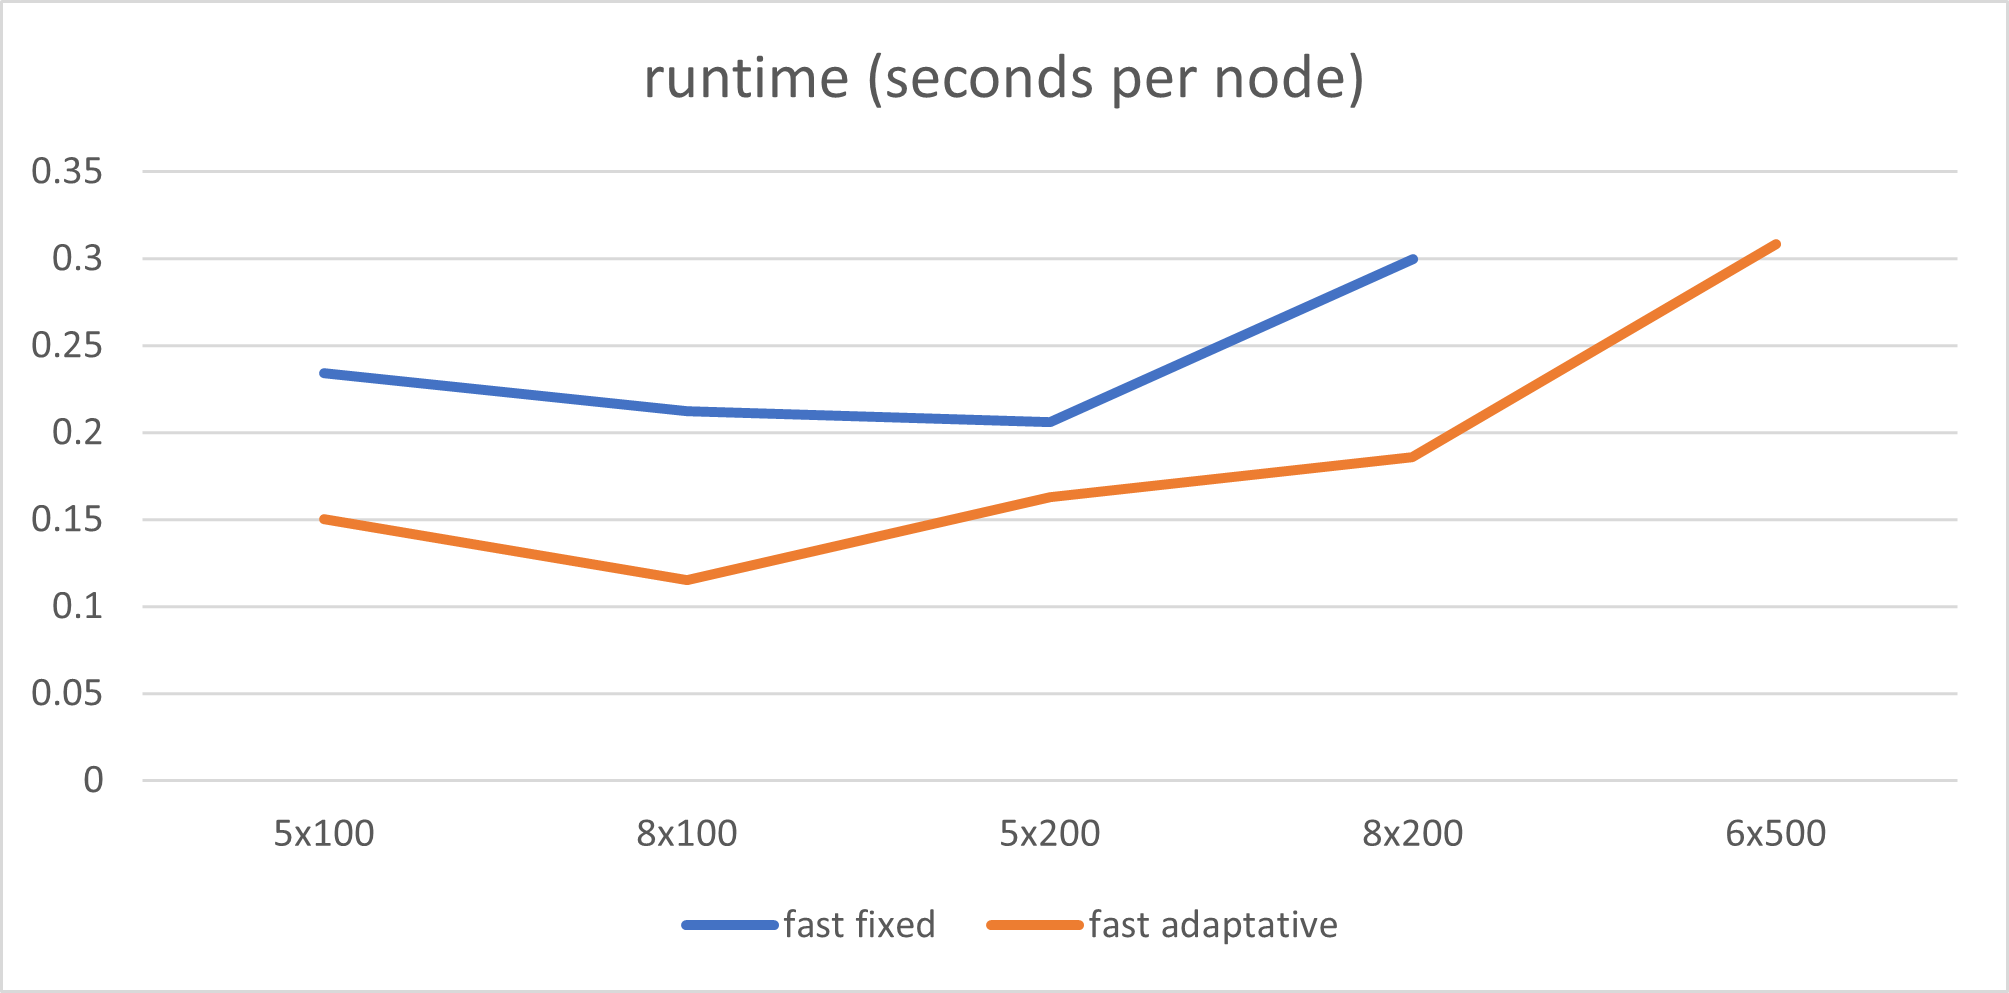
\includegraphics[scale=0.7]{Graph.png}
\end{figure}
\vspace{-0.4cm}

Last, we display the average runtime per number of nodes of both fast adaptive and fast fixed compensation, for the different DNNs considered. The time per node is not constant, but it is still controlled and does not show an exponential blow-up, from 0.1s per node for the smallest DNN to 0.3s per node for the biggest DNN. This indicates that Compensate($K$) can be run on larger DNNs without hitting the same complexity wall as BaB.


\section{Limitations and Discussion}
\label{Discussion}

For DNNs robustly trained, $\alpha$-$\beta$-CROWN and PRIMA are excellent solutions, both very fast and very accurate, usually matching or getting very close \cite{crown} to the upper bound on the $\%$ of verified images \cite{attack}. Compensation strength is not required in these contexts, reason why we did not consider it.

We only considered DNNs with ReLU activation functions in this paper. The reason is that MILP, which is the basic block of Compensate($K$) (and BaB for $\beta$-Crown) can handle the ReLU activation function efficiently. Other activation functions are abstracted in more complex ways, e.g. by PRIMA (unlike $\beta$-CROWN). Still, the compensation paradigm is  orthogonal to the activation function. We believe that studying the compensation strength would be useful with other activation functions as well. We leave that for future work. 

Accuracy of Compensate($K$) is among the highest of the efficient verifiers that do abstraction on values. Runtime, while never blowing-up, can be on the slow side though, in particular for larger DNNs. There are many optimizations possible. The simplest is to run $\alpha$-$\beta$-CROWN first in the pipeline, and only use Compensate($K$) for those images for which $\alpha$-$\beta$-CROWN cannot conclude, possibly using more CPU cores to compute more nodes in parallel. Another simple way is to modify the {\em refined} BaB of $\beta$-CROWN to run Compensate($K$) on more layers than what exact MILP can do, and finish the verification using BaB. More involved would be to modify BaB to branch on unstable ReLU nodes guided by the compensation strength. Also, an analysis of important nodes for the uncertain output nodes could be performed, allowing to compute much faster less accurate bounds for those nodes not important. Last, one could perform a Refinement Abstraction framework similar to \cite{atva}, \cite{elboher}, or \cite{SRGR}.

On the correlation between neurons, which PRIMA encodes explicitly, our results tend to show that it is more efficient to use the compensation strength to abstract the network. Still, considering ReLU nodes exactly tends to be very accurate locally, but less when the source of correlation is many layers away. Few important correlations {\em a la} PRIMA could be kept explicitly as linear constraints in the MILP encoding, helping to reduce the inaccuracies further.




\vspace{-0.2cm}
\section{Conclusion}
\vspace{-0.2cm}

In this paper, we introduced the notion of {\em compensating pairs of paths}, with rationale why such a phenomenon creates inaccuracies hard to handle when verifying DNNs. We proved that this phenomenon is actually explaining entirely the inaccuracies, as in their absence, even the simplest Box abstraction (interval arithmetic) suffices to verify accurately DNNs. We verified experimentally that DNNs learnt in a natural way, harder to verify than robustly trained DNNs, exhibit paths with larger compensating strength. 

Based on this idea of compensating pairs of paths, we proposed abstraction $\MILP_{Z}$ considering a subset $Z$ of the set of unstable ReLU nodes, that we proved to be fully accurate if {\em all} the compensating paths are covered by $Z$. Last, we experimentally showed that choosing $Z$ covering {\em few} paths with the strongest compensations, results in very good accuracy, and runtime which can be favourable in some (but not all) cases. This proves that compensating strength is a promising novel concept which should be further studied to improve DNN verification. We finally proposed several ways to use the compensating strength to optimize current tools in different directions, and leave that as future work.

\newpage

\bibliographystyle{plain}
\bibliography{references}

\newpage

\appendix

\section*{Appendix}

Settings for Hybrid MILP (for Fully Connected DNN, and for CNNs): TO for $\alpha,\beta$-Crown
and number of opens nodes in different layers.



We list some tables and figures comparing $\alpha,\beta$-Crown with other method, from literature.

\subsubsection*{PRIMA} 

PRIMA is one of ERAN's major verifier. Its authors have shown its performance in their paper.

Basically, PRIMA is slightly less accuracy and slower than $\alpha,\beta$-Crown for several networks we considered. Here, we directly use the tables from $\alpha,\beta$-Crown's paper:

\begin{figure*}[h]
	\centering
	\caption{Tables from \cite{crown} to compare $\alpha,\beta$-Crown with earlier verifiers}
	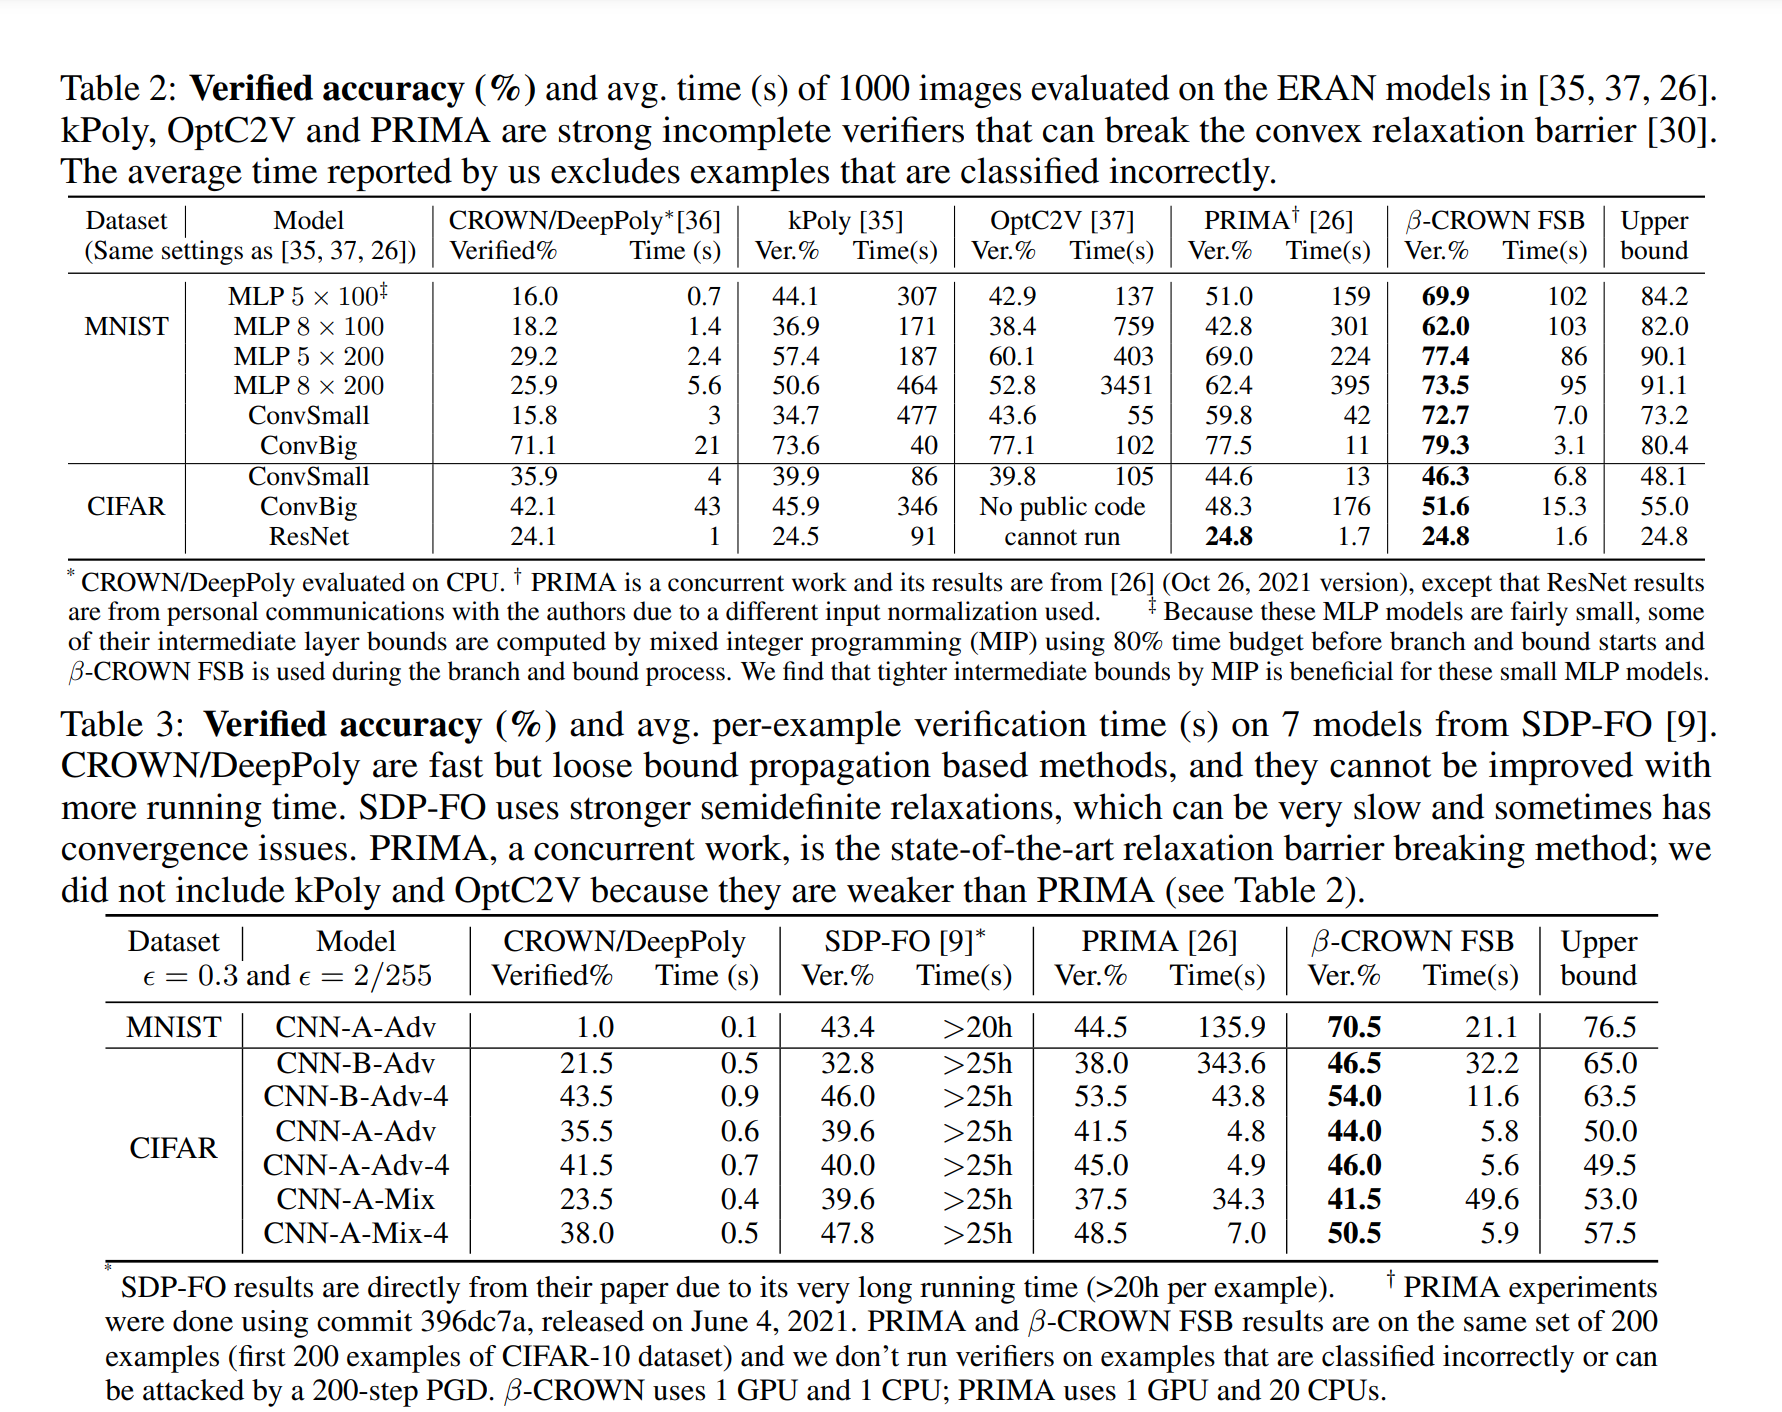
\includegraphics[scale=0.32]{Cronw_PRIMA.png}
\end{figure*}


\subsubsection*{MN-BaB} 


Basically, MN-BaB's performance is close to $\alpha,\beta$-Crown with several kinds of networks. 
\begin{figure}[h]
	\centering
	\caption{A Table from \cite{ferrari2022complete} to compare MN-BaB with $\alpha,\beta$-Crown and other verifiers}
	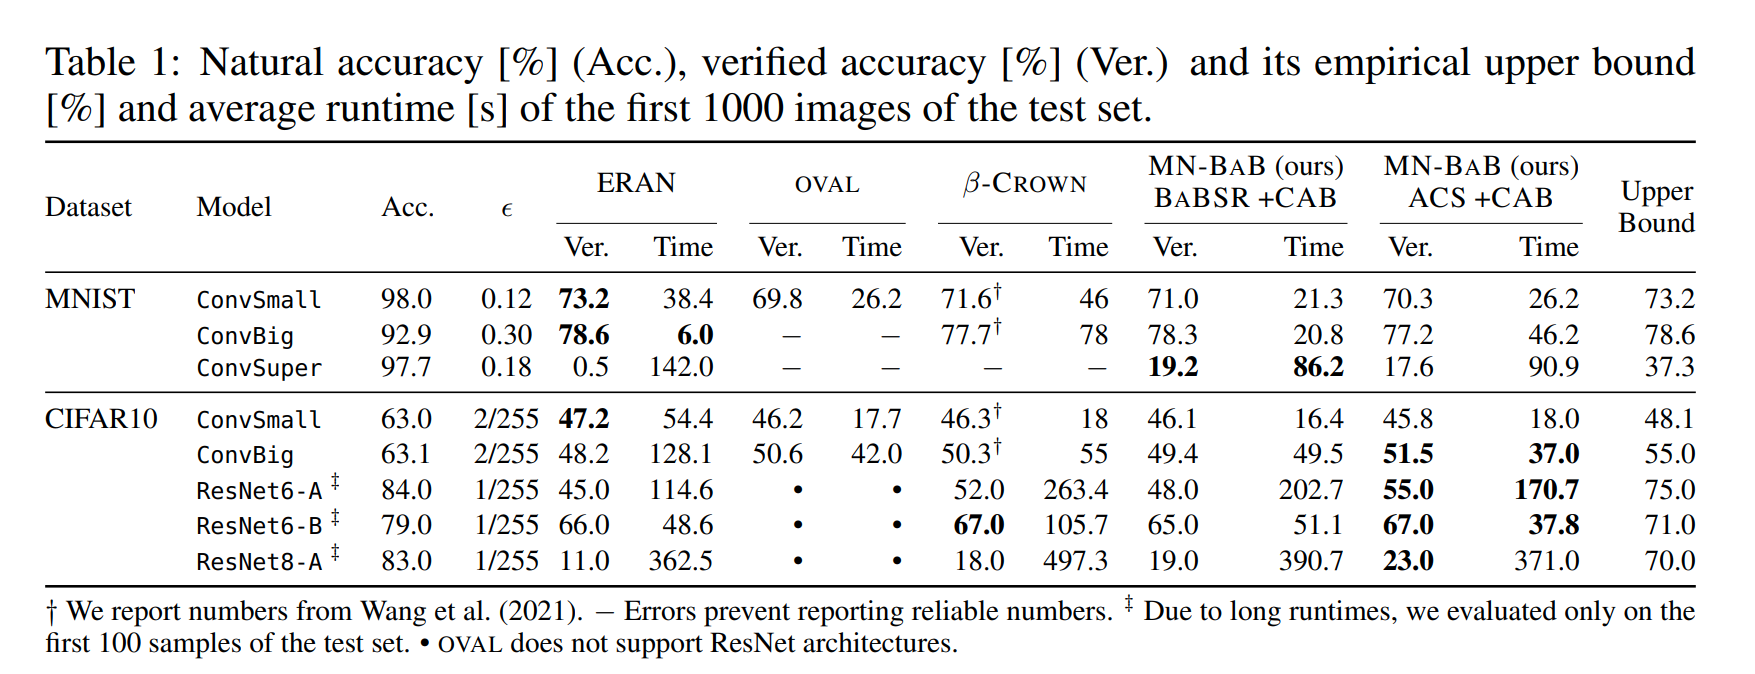
\includegraphics[scale=0.32]{ToMNBAB.png}
\end{figure}

However, the experiments section in their paper does not include those network we focus on. So we run MN-BaB on several networks on our device. The comparison is as follows:

\begin{table}[h]
	\centering
	\begin{tabular}{||l|c|c||c|c||}
		\hline
		Network &  Accuracy & Upper   & MN-BaB &  $\alpha,\beta$-Crown  \\ \hline
		MNIST 6$\times$500 & 99\% & 90\% & $49\%$ & 40 \%    \\
		$\epsilon = 0.035$ & &  &  4995s & 6100s
		\\  \hline
		CIFAR CNN-B-ADV & 99\% & 90\% & $49\%$ & 40 \%    \\
		$\epsilon = 2/255$ & &  &  4995s & 6100s
		\\  \hline
	\end{tabular}
	\caption{}
\end{table}







\subsubsection*{NNenum} 

Similarly, the experiments section in NNenum's paper does not include those network we focus on. So we run NNenum on several networks on our device. 

%As a first step to prove Theorems \ref{th1} and \ref{th2}, 
%we will relax the compensating pairs notion to allows pairs of paths having nodes in common.
%Such a pair is called a {\em weak compensating pair}.
%We will then in a second step prove Theorems \ref{th1} and \ref{th2} for the full definition of compensating pairs of paths.
%
%Let $\cal B$ be a neighbourhood of an input.
%For convenience,
%when the neighbourhood $\cal B$ is clear, 
%we will write $\max(n)$ to denote $\max_{\vx \in \cal B}(\Val_{\vx}(n))$, and $\min(n)$ to denote $\min_{\vx \in \cal B}(\Val_{\vx}(n))$.
%Notice that if $\Val_{\vx}(b)$ is maximal (resp. minimal), 
%then $\Val_{\boldsymbol{x}}(\hat{b})$ also gets maximal (resp. minimal), for $\hat{b}=\texttt{ReLU}(b)$. 
%
%
%We fix a target node $z$.
%We now define the partial influence sign function $S^z$, denoted $S$ when $z$ is clear from the context:
%
%\begin{definition}
%	\label{sign_of_nodes}
%	We define the partial influence sign function $S$ on node $n$: 	
%	\begin{enumerate}
%		\item $S(n)=0$ if all path from $n$ to $z$ have weight $0$; 
%		\item $S(n)=1$ if all path from $n$ to $z$ have non-negative weight, and at least one path has a positive weight; 
%		\item $S(n)=-1$ if all path from $n$ to $z$ have non-positive weight, and at least one path has a negative weight. 
%	\end{enumerate}
%\end{definition}
%
%In general, $S$ may not be defined on every node 
%(e.g. if there is a negative and a positive path from $a$ to $c$). 
%However, if there is no compensating pair of paths, 
%$S$ is defined on all nodes: any node fulfills one of the above cases (1),(2),(3).
%
%For instance for any 3 layer DNN: for an input node $a_i$:
%\begin{enumerate}
%	\item  $S(a_i)=0$ if 
%	for all $b_j, W_{a_i b_j}\cdot W_{b_j c} = 0$
%	
%	
%	\item  $S(a_i)=1$ if for all $b_j, W_{a_i b_j}\cdot W_{b_j c} \geq 0$ and there exists 
%	$j, W_{a_i b_j}\cdot W_{b_j c} > 0$
%	
%	\item $S(a_i)=-1$ if for all $b_j\ W_{a_i b_j}\cdot W_{b_j c} \leq 0$ and there exists 
%	$j, W_{a_i b_j}\cdot W_{b_j c} < 0$ 
%\end{enumerate}
%
%For $b_j$ in the hidden layer, we have $S(b_j)=1,-1,0$ if $W_{b_j c}$ is positive, negative, or 0 respectively. Finally, for the output node $z$, we define $S(z)=1$.
%
%
%
%
%
%\section{Proof of Theorem \ref{th1}}	
%
%
%Assume that there is no (weakly) compensating pair of paths.
%
%
%\begin{lemma}
%	\label{lemma1}
%	Let $L,L'$ be consecutive layers of a DNN without compensation, 
%	$m\in L$ and $n\in L'$. If $W_{m n} \neq 0$ and $S(n) \neq 0$, then 
%	$S(m)=S(n)\mathrm{Sign}(W_{n m})$.
%\end{lemma}
%
%\begin{proof}
%	If $S(n) \neq 0$, then there is a path $\pi$ from $n$ to the output node $z$ with a nonzero weight of the same influence sign as $S(n)$. 
%	So there is a non zero path from $m$ to $z$: $(m n) \pi$, whose influence sign is 
%	$S(n)\mathrm{Sign}(W_{n m})$. As there is no compensation, $S(m)=S(n)\mathrm{Sign}(W_{n m})$.
%	\hfill $\square$
%\end{proof}
%
%
%%For a node $n$, we use $n_s$ to denote $S(n)\cdot n$. 
%%Notice that for $S(n)=1$, $n_s$ gets maximal value whenever $n$ gets maximal value; 
%%while for $S(n)=-1$, $n_s$ gets maximal value whenever $n$ gets minimal value (and vice versa). For $S(n)=0$, $n_s=0$ and thus always reach his minimal and maximal.
%
%Using the concept of influence sign, we introduce input vectors $\vx^{*}, \vx^{\sharp}$: 
%
%\begin{definition}
%We define the following two input vectors $\vx^{*}, \vx^{\sharp}$ in $\cal B$: 
%	\begin{itemize}
%		\item $\vx^{*}$ is the input vector defined in the following way:
%		\begin {itemize}
%		 \item $x^*_{a_i}=\max(a_i)$ if $S(a_i)\in \{0,1\}$, and
%          \item $x^*_{a_i}=\min(a_i)$ otherwise, that is when $S(a_i)=-1$.
%	\end{itemize}
%		
%		\item $\vx^{\sharp}$ is the input vector defined in the following way:
%		\begin{itemize}
%			\item $x^{\sharp}_{a_i}=\min(a_i)$ if $S(a_i)\in \{0,1\}$, and
%			\item $x^{\sharp}_{a_i}=\max(a_i)$ otherwise, that is when $S(a_i)=-1$.
%		\end{itemize}
%	\end{itemize}
%\end{definition}
%
%{Notice that above definitions only involve weights, and do not use bias. As demonstrated by the following lemmas and proofs, our discussion is independent of bias, regardless of whether the bias values are very large or very small.}
%
%We can then prove the following key lemma for Theorem \ref{th1}.
%
%\begin{lemma}
%	\label{lem:key1}
%	\label{lemma2}
%For all $n$ with $S(n)=1$, we have $\val_{\vx^*}(n) = \max(n)$
%and $\val_{\vx^{\sharp}}(n) = \min(n)$.
%For all $n$ with $S(n)=-1$, we have $\val_{\vx^*}(n) = \min(n)$
%and $\val_{\vx^{\sharp}}(n) = \max(n)$. Further, for $L,L'$ two consecutive layers and $n$ on layer $L'$:
%$$\max(n)=\sum_{m \in L, W_{mn}>0}W_{mn} \max(\hat{m}) + \sum_{m \in L, W_{mn}<0}W_{mn} \min(\hat{m}) + bias_n$$
%$$\min(n)=\sum_{m \in L, W_{mn}>0}W_{mn} \min(\hat{m}) + \sum_{m \in L, W_{mn}<0}W_{mn} \max(\hat{m}) + bias_n$$
%
%\end{lemma}
%
%\begin{proof}
%	We prove this lemma by induction on layers. For input layer, this is true by definition. Suppose this lemma is true up to layer $L_i$, we need to show this for layer $L_{i+1}$. Let $n$ be a node in layer $L_{i+1}$, then by definition, we have the following equation: \begin{align*}
%		\val_{\vx}(n) = \sum_{m\in L}W_{m n}\val_{\vx}(\hat{m})) + bias_n.
%	\end{align*}
%	
%	By induction hypothesis, when input vector is $\vx^{*}$, for every $m$, if $S(m)=1$, then $\Val_{\vx^*}(\hat{m})=\max(\hat{m})$ and if $S(\hat{m})=-1$, then $\Val_{\vx^*}(\hat{m})=\min(\hat{m})$. Assume that $S(n)=1$. By applying Lemma \ref{lemma1} and the induction hypothesis:
%	\begin{align*}
%		\val_{\vx^*}(n) = \sum_{m \in L_i, W_{mn}>0}W_{mn} \max(\hat{m}) + \sum_{m \in L_i, W_{mn}<0}W_{mn} \min(\hat{m}) + bias_n\\
%	\end{align*}
%	
%
%
%	Further, we have the following inequality:
%	\begin{align*}
%		\max(n)\leq & \sum_{m \in L_i, W_{mn }>0}W_{mn} \max(\hat{m}) + \sum_{m \in L_i, W_{mn}<0}W_{mn} \min(\hat{m}) + bias_n\\
%		\leq & \val_{\vx^*}(n)
%	\end{align*}
%	
%	%If $S(m)=1$, then by Lemma \ref{lemma1}, $W_{mn}>0$; if $S(m)=-1$, then $W_{mn}<0$; if $S(m)=0$, then $W_{mn}=0$.
%	
%	By definition of $\max$, we have $\val_{\vx^*}(n) \leq \max(n)$.
%	Combining the 2 formulas, we obtain $\max(n)=\Val_{\vx^*}(n)$. 
%	
%	We prove similarly that $\min(n)=\Val_{\vx^\sharp}(n)$,
%	and the case $S(n)=-1$. This concludes the induction. 
%\end{proof}
%
%{ As we mentioned earlier, this proof does not have any requirements on the bias.}
%
%\iffalse
%	As direct corollary of Lemma \ref{lem:key1}, we obtain:
%	
%	\begin{corollary}
%		\label{cor1}
%		$$\max(c)=\sum_{b \in L, W_{bc}>0}W_{bc} \max(\hat{b}) + \sum_{b \in L, W_{bc}<0}W_{bc} \min(\hat{b}) + bias_c$$
%		$$\min(c)=\sum_{b \in L, W_{bc}>0}W_{bc} \min(\hat{b}) + \sum_{b \in L, W_{bc}<0}W_{bc} \max(\hat{b}) + bias_c$$
%	\end{corollary}
%	
%\fi
%	
%	%Notice that for all $x$, for either $S(c)=1$ or $S(c)=-1$, these two bounds are found in Lemma \ref{lemma2},
%	%from configuration $\boldsymbol{x}^*$ and $\boldsymbol{x}^\sharp$.
%	
%	
%	
%	
%	
%	\subsubsection*{Bounds generated by Value Abstraction}
%
%	\smallskip
%	
%	Let $[\alpha_n,\beta_n]$ be the bounds generated by the Box abstraction.
%	We show that these bounds are exact when there is no (weak) compensating pairs of paths, i.e. for all node $n$ of the DNN, we have $\alpha_n=\min(n)$ and $\beta_n=\max(n)$.
%
%\begin{proof}
%	 We show that inductively. The initialization is obvious as Box Abstraction is always exact for the first layer.
%
%	Let $n$ be node of the DNN. We set the target $z=n$ and consider the influence sign function $S^z=S^n=S$ corresponding to that node. By definition, $S(n)=1$. 
%	
%	The Box abstraction computes its upper bound using:
%	$$\beta_n= \sum_{W_{mn}>0} W_{mn} \beta_{\hat{m}} + \sum_{W_{mn}<0} W_{mn} \alpha_{\hat{m}} + bias_n$$
%
%	By induction hypothesis, we have 
%		$\beta_{\hat{m}}=\max(\hat{m})$ and
%		$\alpha_{\hat{m}}=\min(\hat{m})$, thus 
%		applying the second part of Lemma \ref{lem:key1}, we obtain
%		$\beta_n=\max(n)$.
%		
%		Similarly, we obtain $\alpha_n=\min(n)$.
%		
%		Consider now $\alpha_{\hat{n}},\beta_{\hat{n}}$.
%		If $\alpha \leq 0$ then $\alpha_{\hat{n}}=0=\max(\hat{n})$.
%		Otherwise, $\alpha_{\hat{n}}=\alpha_n=\max(\hat{n})$.
%		In both case it is exact.
%
%		Similarly, if $\beta_n=\max(n)<0$, 
%		then $\beta_{\hat{n}}=\max(\hat{n})=0$, 
%		and otherwise 
%		$\beta_{\hat{n}}=\max(\hat{n})=\beta_n=\max(n)$.
%		
%		Hence we have equality pre and post activation function.
%			\end{proof}
%	
%
%
%This shows the statement of Theorem 1 with the weaker statement that there is no weak compensating pairs of paths.
%
%	
%	
%	\subsubsection*{From weak to normal}
%	
%	\begin{lemma}
%		If a DNN has no compensating pair, then it also does not have weak compensating pair from an input node to the output node.
%	\end{lemma}
%	
%	\begin{proof}
%		By contradiction, if there is a weak compensating pair of two paths, $\rho_1,\rho_2$, 
%		then consider the common nodes by increasing layer $n_1 \cdots n_k$ in $\rho_1,\rho_2$ (including the initial and final nodes).
%		Assume that there is no compensating pair.
%		It means that all the segment of $\rho_1,\rho_2$ from $n_i$ to $n_{i+1}$ have the same influence sign (they have no nodes in common but the initial and final nodes).
%		Hence $\rho_1$ and $\rho_2$ have the same influence sign, a contradiction with $\rho_1,\rho_2$ being a weakly compensating pair. 
%	\end{proof}
%	
%	This finishes the proof of Theorem \ref{th1}.
%	
%	
%
%
%
%
%
%
%\newpage
%
%
%
%
%
%	
%
%
%
%
%
%			
%\section{Proof of Theorem \ref{th2}}
%			
%			In this section, we will prove theorem \ref{th2}. We first prove the following weaker theorem:
%			
%			\begin{theorem} \label{thm:2}	
%				Suppose $\mathcal{D}$ is a DNN with a unique output node $z$.
%				Let $X$ be the set of nodes $n$ such that there is a weak compensating path 
%				passing by $n$ (except its source and target nodes).
%				Then $\MILP_X$ computes the exact bounds $[\alpha,\beta]$ for $z$,
%				i.e. $\alpha=\min(z)$ and $\beta=\max(z)$.
%			\end{theorem}
%			
%			
%			\subsection{Proof of Theorem \ref{thm:2}}
%			
%			\begin{definition}
%				We define a partition of the set $A$ of input nodes as $A_{zero} \sqcup A_{pure}\sqcup A_{open}$, with:  
%				\begin{itemize}
%					\item $A_{zero}= \{a \mid \forall \text{ path $\rho$ from $a$ to } z, weight(\pi)=0\}$.
%	
%					\item $a_k \in A_{pure}$  if $a \notin A_{zero}$ and either
%					\begin{enumerate}
%						\item every path from $a_k$ to $z$ has weight $\geq 0$, or
%						\item every path from $a_k$ to $z$ has weight $\leq 0$. 
%						
%					\end{enumerate}
%					Hence, $a_k$ is not a source of a weak compensating pair. We denote 
%					$A_{pure}$ by $I$ for short.
%					\item $a_k \in A_{open}$ iff $a_k \notin A_{pure} \sqcup A_{zero}$, that is there exists two paths $\rho,\rho'$ from $a_k$, one with positive and one with negative weight. 	We denote $A_{open}$ by $J$ for short.
%				\end{itemize}
%			\end{definition} 
%			
%
%			
%			\begin{lemma} \label{lem:open_node_2}
%				A node $b$ in a hidden layer will not be on a weak compensating path if and only if one of the following happens:
%				\begin{enumerate}
%					\item Any path from $b$ to the output node $z$ has a weight $0$, and we use $weight({bz})=0$ to denote this case, or
%					\item For every input node $a_j\in J$, every path from $a_j$ to $b$ has a weight of $0$. We use $weight({a_jb})=0$ to denote this case.
%				\end{enumerate}
%				
%			\end{lemma}
%			
%			We denote $B_{zero}$ the set of nodes $b$ that case 1 holds, and denote $B_{pure}$ the set of nodes $b$ such that case 2 holds but case 1 does not hold.
%			We denote $B_{open}$ the set of all nodes $b$ in a weak compensating path (remaining cases).
%			
%		{ 	Similarly, above definitions $A_{zero},A_{open}, A_{pure}$ and $B_{zero},B_{open},B_{pure}$ do not consider bias, and any kind of bias will not affect our theorem.}
%		
%		\begin{figure}[h]
%			\centering
%			\begin{tikzpicture}[>=stealth, node distance=2cm]
%				% Input nodes (two types)
%				\node[circle, draw, minimum size=0.5cm] (input1) at (-1,0) {$a_0$};
%				\node[circle, draw, minimum size=0.5cm] (input2) at (-2,0) {$a_1$};
%				\node[circle, draw, minimum size=0.5cm] (input3) at (-4,0) {$a_2$};
%				
%				\node[circle, draw, minimum size=0.5cm] (input4) at (-5,0) {$a_3$};
%				\node[circle, draw, minimum size=0.5cm] (input5) at (-7,0) {$a_4$};
%				\node[circle, draw, minimum size=0.5cm] (input6) at (-8,0) {$a_5$};
%				
%				\draw[draw=black, dashed] (-1.5,0) ellipse (1.35 and 0.75);
%				\node[below] at (-1.5,-0.75) {$A_{zero}$};
%				
%				\draw[draw=black, dashed] (-2,2) ellipse (0.75 and 0.75);
%				\node[right] at (-1,2) {$B_{zero}$};
%				
%				% Hidden layer nodes
%				
%				\node[circle, draw, minimum size=0.5cm, fill=blue!20] (hidden1) at (-2,2) {$n_0$};
%				
%				\node[circle, draw, minimum size=0.5cm, fill=blue!20] (hidden2) at (-4,2) {$n_1$};
%				\node[circle, draw, minimum size=0.5cm, fill=blue!20] (hidden3) at (-5,2) {$n_2$};
%				
%				\node[circle, draw, minimum size=0.5cm, fill=blue!20] (hidden4) at (-7,2) {$n_3$};
%				\node[circle, draw, minimum size=0.5cm, fill=blue!20] (hidden5) at (-8,2) {$n_4$};
%				
%				
%				
%				\draw[draw=black, dashed] (-4.5,0) ellipse (1.35 and 0.75);
%				\node[below] at (-4.5,-0.75) {$A_{pure}$};
%				
%				
%				\draw[draw=black, dashed] (-7.5,0) ellipse (1.35 and 0.75);
%				\node[below] at (-7.5,-0.75) {$A_{open}$};
%				
%				
%				
%				\draw[draw=black, dashed] (-4.5,2) ellipse (1.35 and 0.75);
%				\node[left] at (-3.5,3) {$B_{pure}$};
%				
%				
%				\draw[draw=black, dashed] (-7.5,2) ellipse (1.35 and 0.75);
%				\node[left] at (-8.5,1.5) {$B_{open}$};
%				
%				
%				
%				% Output node
%				\node[circle, draw, minimum size=0.8cm, fill=red!20] (output) at (-5,4) {$z$};
%				
%				
%				% connections
%				
%				\draw[->] (input1) -- (hidden1);
%				
%				\draw[->] (input3) -- (hidden5);
%				
%				\draw[->] (input4) -- (hidden4);
%				
%				
%				%		% Connect input to hidden layer
%				\foreach \i in {3,4} {
%					\foreach \h in {3,2} {
%						\draw[line width=1.5pt, ->] (input\i) -- (hidden\h);
%					}
%				}
%				
%				
%				\foreach \i in {5,6} {
%					\foreach \h in {4,5} {
%						\draw[->] (input\i) -- (hidden\h);
%					}
%				}
%				%		
%				% Connect hidden layer to output
%				\foreach \h in {2,3} {
%					\draw[line width=1pt,->] (hidden\h) -- (output);
%				}
%				
%				\foreach \h in {4,5} {
%					\draw[->] (hidden\h) -- (output);
%				}
%				
%				%\		% Input label
%				\node[left=0.7cm of input6] {Input Layer};
%				
%				% Hidden label
%				\node[left=0.7cm of hidden5] {Hidden Layer};
%				
%				% Output label
%				\node[left=0.5cm of output] {Output Layer};
%			\end{tikzpicture}
%			\caption{Definitions in the proof of Theorem \ref{th2}}
%			\label{fig:neural_network_types_simplified}
%		\end{figure}
%			
%			\begin{proof}
%				First, we show that if one of case 1, 2 happens, then $b$ will not be in a weak compensating pair. If 1), it is obvious. For 2, we reason by contradiction: assume there is a pair of weak compensating paths 	$(\pi,\pi')$ starting with $a$, with $b$ in $\pi$ and weight$(\pi) > 0$. It means that $a \in J$. This is a contradiction as 2) $weight({a_j,b})=0$ implies weight$(\pi)=0$.
%				
%				Second, we show that if neither 1 nor 2 hold, then $b$ will be in a weak compensating path.
%				Because 2) does not hold, there exists $a_j \in J$ with $weight({a_j,b}) \neq 0$, say $>0$.
%				Because 1) does not hold, $weight({b,z}) \neq 0$, say $>0$.
%				Now, by definition of $J$, there is a pair of weak compensating paths $\pi,\pi'$ 
%				from $a_j$ to $z$, say with $\pi'$ with weight $<0$.
%				Then two paths $(a_j,b,z)$ and $\pi'$ also form a weak compensating pair.
%			\end{proof}
%			
%						
%			
%			\begin{lemma}\label{lem:subnetwork}
%				$I \cup B_{pure} $ forms a sub-network, denoted $D_I$. That is, 
%				for $n \in B_{pure}$, for every path $\rho$ from $m$ to $n$
%				either $m \in B_{pure}\cup I$ or $weight(\rho)=0$.
%				Further, in $D_I$, there is no (weakly) compensating pair.
%			\end{lemma}
%
%			
%
%			
%			\begin{proof}
%				This is simply because for a node $c\in B_{pure}$ in a hidden layer or the output layer, for a node $b$ in one layer before, if $b\notin B_{pure}\cup I$, then:
%				
%				1. if $b\in J$, by definition, $W_{bc}=0$.
%				
%				2. if $b\in B_{open}$, then $W_{bc}=0$; otherwise there exists $<a_j,b,c>$ a path from $a_j\in J$ to $c$ with a nonzero value, a contradiction.
%				
%				3. if $b\in B_{zero}$, then $W_{bc}=0$; otherwise there exists $<b,c,z>$ a path from $b$ to $z$ the output node with a nonzero value, a contradiction. 
%			\end{proof}
%			
%			
%			
%			For an input $\vx$ and a subset $S$ of input nodes, we denote by 
%			$\boldsymbol{x}_S$ to refer the input vector $\langle x_{a_k}\rangle_{a_k\in S}$. We use $\boldsymbol{x}_I\oplus \boldsymbol{x}_J = \boldsymbol{x}$ and 
%			$\Val_{\boldsymbol{x}_I,\boldsymbol{x}_J} (z)=\Val_{\boldsymbol{x}}(z)$. 
%			
%			
%			Invoking Lemma \ref{lem:subnetwork}, we can apply Theorem 1 on $D_I$, and obtain two input vectors $\boldsymbol{x}_I^*,\boldsymbol{x}_I^{\sharp}$ on $I$
%			minimizing and maximizing all the nodes in $D_I$.
%
%			\smallskip
%
%		
%			Recall the influence sign function of nodes from Definition \ref{sign_of_nodes}. 
%			Because weakly compensating paths are allowed, the influence sign function is no longer defined on all nodes. $S$ is defined for all nodes from which there is no weakly compensating pairs of paths to $z$. In particular, $S$ is defined on all nodes of $I$.
%
%			\begin{lemma}\label{lem:sign}
%				Let $m,n$ be two nodes, such that $S$ is defined on $m$ and there is a path $\rho$ with non zero weight to a node $n$. Then $S$ is defined on $n$
%				 (there is no compensating pair of paths from $n$ to $z$).
%				Further, $S(n)= Sign(weight(\rho)) S(m)$.
%			\end{lemma}
%			
%			\begin{proof}
%				By contradiction, assume that there exists two paths $\rho_1,\rho_2$ from 
%				$n$ to $z$ with (strictly) different influence signs. The pair $\langle a_i,n\rangle \cdot \rho_1$ and $\langle a_i,n\rangle \cdot \rho_2$ is compensating, a contradiction with $a_i\in I$. 
%			\end{proof}
%
%			Hence, for all node $n$, either $S$ is defined on $n$, or 
%			$n$ depends only upon input nodes in $J$.
%			Let us call $D_J$ the set of such nodes which only depends upon nodes in $J$.
%			$D_J$ forms a sub-network.
%			$D_J$ contains the set of all nodes from which there is a weakly compensating pair of paths to $z$.
%			By definition, for any $b\in D_J$, either $b\in B_{open}$, or $b$ is a constant node: any path from any input node must have zero weight to it.
%			For a node $b$ for which $S$ is undefined, $b$ thus only depends on $J$; so, if $\boldsymbol{x}_J$ is fixed, then the value of $b$ will be fixed.
%			Notice that $D_I \sqcup D_J$ does not cover the DNN entirely in general.
%			
%			
%			
%			\begin{lemma} \label{lem:reach_max_2}
%				Let $n$ be a node on which $S$ is defined. If $S(n)=1$,
%				for any valuation $\boldsymbol{x}^0_J$,	we have: 
%				$$\max_{\boldsymbol{x}_I} (\Val_{\boldsymbol{x}_I,\boldsymbol{x}^0_J}(b)) =  \Val_{\boldsymbol{x}_I^*,\boldsymbol{x}^0_J}(b).$$
%				
%				$$\min_{\boldsymbol{x}_I} (\Val_{\boldsymbol{x}_I,\boldsymbol{x}^0_J}(b)) =  \Val_{\boldsymbol{x}_I^{\sharp},\boldsymbol{x}^0_J}(b).$$
%				
%				
%				If $S(b)=-1$, 
%				$$\max_{\boldsymbol{x}_I} (\Val_{\boldsymbol{x}_I,\boldsymbol{x}^0_J}(b)) =  \Val_{\boldsymbol{x}_I^{\sharp},\boldsymbol{x}^0_J}(b).$$
%				
%				$$\min_{\boldsymbol{x}_I} (\Val_{\boldsymbol{x}_I,\boldsymbol{x}^0_J}(b)) =  \Val_{\boldsymbol{x}_I^{*},\boldsymbol{x}^0_J}(b).$$	
%			\end{lemma}
%			
%			\begin{proof}	
%				Fix an input vector $\boldsymbol{x}^0_J$.
%				This also fixes the values in $D_J$.
%				Consider the DNN $D'$ with input nodes $a_i\in I$, where all the 
%				edges from $m \in D_J$ to $n$ are replaced by a bias (equals to the weight of the edge times the fix value $\val_{\boldsymbol{x}^0_J}(m)$) for $n$ (we sum all these bias for a neuron $n$).
%				We denote $\val'$ values of nodes in this DNN $D'$.
%				 
%				We have $\Val_{\boldsymbol{x}_I,\boldsymbol{x}^0_J}(z) = \val'_{\boldsymbol{x}_I}(z)$.
%				In the simplified $D'$, there is no weakly compensating path to $z$ because 
%				$D_J$ contains all the source of weakly compensating path to $z$.
%				Therefore we can apply Lemma \ref{lem:key1} to get that 
%				$\val'_{x_I}(z)$ reaches its maximal value for $\boldsymbol{x}_I=\boldsymbol{x}_I^*$, and conclude by using $\Val_{\boldsymbol{x}_I,\boldsymbol{x}^0_J}(z) = \val'_{\boldsymbol{x}_I}(z)$. The case for min is similar. 
%			\end{proof}
%			
%			From Lemma \ref{lem:reach_max_2}, we immediatly obtain the following corollary:
%
%			\begin{corollary}
%				\label{corr:main}
%			For a node $b$ with $S(b)=1$:
%		
%			$$\max(b)=\max_{\vx_J} \val_{\vx^{\star}_I,\vx_J}(b)$$
%			$$\min(b)=\min_{\vx_J} \val_{\vx^{\sharp}_I,\vx_J}(b)$$
%			and for $S(b)=-1$:
%	
%			$$\max(b)=\max_{\vx_J} \val_{\vx^{\sharp}_I,\vx_J}(b)$$
%			$$\min(b)=\min_{\vx_J} \val_{\vx^{\star}_I,\vx_J}(b)$$
%			\end{corollary}
%			
%	
%			
%
%
%			%\subsection{$\MILP_X$ is accurate}
%			
%			
%
%
%
%
%
%			%We want to show that $\beta= \max(z)$. 
%			%As the MILP abstraction is a sound over-approximation, it suffices to show that %$\beta\leq \max (z)$.
%			%The case for $\alpha$ is similar.
%			
%			
%			%\begin{lemma}
%			%	Both $D_I$ and $D_J$ are accurate in the sense that for any $b$ in $D_I$ or %$D_J$, $\UB(b)=\max(b)$ and $\LB(b)=\min(b)$.
%			%\end{lemma}
%			
%			%\begin{proof}
%			%	For $D_I$, it is because of no compensating as proved in the first section. %For $D_J$, it is because all nodes are either opened or constants. 
%			%\end{proof}
%			
%			
%			%\begin{definition} Assume $\boldsymbol{x}^0_I\oplus \boldsymbol{x}^0_J$ is a input vector, and $b$ is node in hidden layers or output layer.
%			%
%			%	1. For a given vector $\boldsymbol{x}$ , $\B_{\boldsymbol{x}^0_I, \boldsymbol{x}^0_J, \boldsymbol{x}}(b)$ is the value of $b$ in the MILP model for values $\boldsymbol{x}^0_I, \boldsymbol{x}^0_J, \boldsymbol{x}$.
%			%\end{definition}
%\iffalse			
%			For input vectors $\boldsymbol{x}^0_I,\boldsymbol{x}^0_J$, let $\UB_{\boldsymbol{x}^0_I,\boldsymbol{x}^0_J}(b)$ be the upper bound in the above fixed formulation and framework while the input $\boldsymbol{x}^0_I,\boldsymbol{x}^0_J$ is fixed: that is, besides the constraints in above MILP models, we add new constraints $\boldsymbol{x}_I,\boldsymbol{x}_J=\boldsymbol{x}^0_I,\boldsymbol{x}^0_J$. We  define $\LB_{\boldsymbol{x}^0_I,\boldsymbol{x}^0_J}(b)$ similarly for $\LB$ lower bound. For them, we have the following lemma:
%			
%			\begin{lemma} In an MILP formulation, for a node $c$ in a hidden layer or output layer:
%				
%				1. $\UB(b)=\max_{\boldsymbol{x}^0_I,\boldsymbol{x}^0_J}\UB_{\boldsymbol{x}^0_I,\boldsymbol{x}^0_J}(c)$. 
%				
%				2. $\LB(b)=\min_{\boldsymbol{x}^0_I,\boldsymbol{x}^0_J}\LB_{\boldsymbol{x}^0_I,\boldsymbol{x}^0_J}(c)$. 
%			\end{lemma}
%			
%			\begin{proof}
%				This is by the definition of MILP formulation and $\UB_{\boldsymbol{x}^0_I,\boldsymbol{x}^0_J}, \LB_{\boldsymbol{x}^0_I,\boldsymbol{x}^0_J}$. 
%			\end{proof}
%			
%	
%			
%			
%		%We will prove this by induction on layers from the first hidden layer to the output layer. More specifically, we will prove the following lemmas:
%			
%	
%
%		\begin{lemma} \label{lem:main}
%				For any node $c$ in a hidden layer or the output layer, if $c\notin B_{zero}$, then:		\begin{enumerate}
%					\item for any fixed $\boldsymbol{x}^0_J$, when  $\boldsymbol{x}_I=\boldsymbol{x}^*_I$, the value for $c$ in the MILP model is a fixed number, and naturally $\UB_{\boldsymbol{x}^*_I,\boldsymbol{x}^0_J}(c)=\LB_{\boldsymbol{x}^*_I,\boldsymbol{x}^0_J}(c)$. The same is true for $\boldsymbol{x}^\sharp_I$.
%					
%					\item for any fixed $\boldsymbol{x}^0_J$, if $S(c)=1$, then $$\max_{\boldsymbol{x}_I} \UB_{\boldsymbol{x}_I,\boldsymbol{x}^0_J}(c)=\UB_{\boldsymbol{x}^*_I,\boldsymbol{x}^0_J}(c)= \Val_{\boldsymbol{x}^*_I,\boldsymbol{x}^0_J}(c) = \max_{\boldsymbol{x}_I} \Val_{\boldsymbol{x}_I,\boldsymbol{x}^0_J}(c).$$ The similar for $S(c)=-1$, $\langle \LB,\min\rangle$, $x^\sharp_I$: we can change two of them at the same time.
%					
%					\item Therefore, $\UB(c)=\max(c)$ and $\LB(c)=\min(c)$.
%				\end{enumerate}
%				
%				
%				
%			\end{lemma}
%			
%
%
%			\begin{proof}
%				We prove this lemma by induction on layers. For first hidden layer $L_1$, it is obvious. Suppose we have proved part 1,2,3 up to layer $L_i$, then for layer $L_{i+1}$, suppose $c$ is a node in this layer. 
%				
%				(1)	If $S(c)$ is undefined, then by previous discussion, $c$ is in a sub-network from $J$ with all nodes opened; and if $\boldsymbol{x}_J=\boldsymbol{x}_J^0$ is fixed, then in the MILP model, the value for $c$ is also fixed. 
%				
%				If $S(c)$ is defined, then consider all $b$ such that $W_{bc}\neq 0$. First, $b$ cannot in $B_{zero}$; so by induction hypothesis, the value of $b$ is fixed under $\boldsymbol{x}^*_I,\boldsymbol{x}^0_J$ in MILP model. 
%				
%				
%				
%				If $b\in B_{open}$, the term is $W_{bc}\ReLU(b)$. We know then by induction hypothesis, the value for $b$ in MILP is a fixed value. Then the term $W_{bc}\ReLU(b)$ is also a fixed number.  
%				
%				If $b\in B_{pure}$, the term is $W_{bc}\mathrm{AppB}(b)$ ($\mathrm{AppB}$ is the LP approximation domain of $\ReLU$) and either $S(b)$ is undefined and $b$ is a constant in the network and so is in the MILP model (trivial case), or $S(b)$ is defined. 
%				
%				Then by induction hypothesis for all 1, 2 and 3 parts,  the value of $b$ in the model is fixed (part 1), and it is equal to $\max_{\boldsymbol{x}_I} \Val_{\boldsymbol{x}_I,\boldsymbol{x}^0_J}(c)$ or $\min_{\boldsymbol{x}_I} \Val_{\boldsymbol{x}_I,\boldsymbol{x}^0_J}(c)$ (by part 2, depending on $S(b)$). Since $b$ only depends on $I$, this value also equal to $\max_{\boldsymbol{x}_I} \Val_{\boldsymbol{x}_I}(c)$ or $\min_{\boldsymbol{x}_I} \Val_{\boldsymbol{x}_I}(c)$, and by induction hypothesis on part 3, equal to $\UB(b)$ or $\LB(b)$. For either of them, $\mathrm{AppB}(b)$ will be fixed value. Hence, in this case, the term $W_{bc}\mathrm{AppB}(b)$ is also a fixed number.
%				
%				Therefore, in the MILP model, $c$ is a sum of terms that are all fixed numbers. Hence $c$ is a fixed number.
%				
%				(2) If $S(c)=1$, then we have the following:	\begin{align*}
%					\mathrm{UB}_{\boldsymbol{x}^0_J,\boldsymbol{x}^0_I}(c) \leq constant + \sum_{b\in B_{open}\cap l_i} W_{bc}\ReLU(\B_{\boldsymbol{x}^0_I,\boldsymbol{x}^0_J}(b)) + \sum_{b\in B_{pure}\cap l_{i}} W_{bc} \mathrm{AppB}(\B_{\boldsymbol{x}^0_I,\boldsymbol{x}^0_J}(b)),
%				\end{align*}where $\B$ means one of $\UB$ or $\LB$ depending on the influence sign of $W_{bc}$: if $W_{bc}$ is positive, then $\UB$, otherwise $\LB$. Notice that all $b$ displayed are that $S(b)$ defined, because if $S(b)$ undefined, then for fixed $\vx_J$, value of $b$ is fixed and will be put into the constant.
%				
%				Now by induction hypothesis part 2, if $S(b)=1$, then $\UB_{\boldsymbol{x}^*_I,\boldsymbol{x}^0_J}(b)=\max_{\vx_I}\UB_{\boldsymbol{x}^*_I,\boldsymbol{x}^0_J}(b)$; and if $S(b)=-1$, $\LB_{\boldsymbol{x}^*_I,\boldsymbol{x}^0_J}(b)=\min_{\vx_I}\LB_{\boldsymbol{x}^*_I,\boldsymbol{x}^0_J}(b)$. Moreover, since $S(c)=1$, $S(b)$ and $W_{bc}$ have the same influence sign. And both $\ReLU$ and $\mathrm{AppB}$ are non-decreasing functions. Combining all these facts, we have:\begin{align*}
%					\mathrm{UB}_{\boldsymbol{x}^0_J,\boldsymbol{x}^0_I}(c)\leq 
%					&constant + \sum_{b\in B_{open}\cap l_i} W_{bc}\ReLU(\B_{\boldsymbol{x}^*_I,\boldsymbol{x}^0_J}(b)) + \sum_{b\in B_{pure}\cap l_{i}} W_{bc} \mathrm{AppB}(\B_{\boldsymbol{x}^*_I}(b))\\
%					= & \mathrm{UB}_{\boldsymbol{x}^0_J,\boldsymbol{x}^*_I}(c). 
%				\end{align*}  This is the first equal.
%				
%				The second is simply because $\UB_{\boldsymbol{x}^*_I,\boldsymbol{x}^0_J}(c)\geq \Val_{\boldsymbol{x}^*_I,\boldsymbol{x}^0_J}(c)\geq\LB_{\boldsymbol{x}^*_I,\boldsymbol{x}^0_J}(c)$.	The third equal is proved in last subsection, Lemma \ref{lem:reach_max_2}. The case $S(c)=-1$ is similar. This is for part 2.
%				
%				(3) Once we have part 2, we will have that for any fixed $\boldsymbol{x}^0_J$, $$\max_{\boldsymbol{x}_I} \UB_{\boldsymbol{x}_I,\boldsymbol{x}^0_J}(c)= \max_{\boldsymbol{x}_I} \Val_{\boldsymbol{x}_I,\boldsymbol{x}_J}(c).$$ Therefore, $\max_{\boldsymbol{x}_I,\boldsymbol{x}_J} \UB_{\boldsymbol{x}_I,\boldsymbol{x}_J}(c)= \max_{\boldsymbol{x}_I,\boldsymbol{x}_J} \Val_{\boldsymbol{x}_I,\boldsymbol{x}_J}(c)$ and this is to say $\UB(c)=\max(c)$. This is what we want to show, and the same result holds for lower bound and minimal value. This is for part 3. 
%
%			\end{proof}
%
%	\fi
%
%
%
%	We denote by $X=B_{open}$, and consider $\MILP_{X}$.
%	Let $[\alpha,\beta]$ be the bounds computed by $\MILP_{X}$ for the target node $z$. We are now ready to finish the proof of Theorem \ref{thm:2}.
%
%			
%\begin{proof}[Proof of Theorem \ref{thm:2}]
%	We show that $\beta=\max(z)$.
%
%	We fix the input vector $\vx^*_I$ for input $I$.
%	This also fixes the values in $D_I$.
%	Consider the DNN $D'$ with input nodes $J$, where all the 
%	edges from $m \in D_I$ to $n$ are replaced by a bias (equals to the weight of the edge times the fix value $\val_{\boldsymbol{x}^*_I}(m)$) for $n$ (we sum all these bias for a neuron $n$). We denote $\val'$ values of nodes in this DNN $D'$.
%		 
%	We have $\val'_{\boldsymbol{x}_J}(n)=\Val_{\boldsymbol{x}^*_I,\boldsymbol{x}_J}(n)$ 
%	for every node $n$ of $D'$. All the ReLU nodes of $D'$ are in $X$, by definition of $X$.
%Thus $\MILP_X$ will be fully accurate in $D'$. Let $\beta'$ denote its upper bound.
%We have $\beta'=\max_{\vx{_J}} (\val'_{\vx_{J}}(z)) = 
%\Val_{\boldsymbol{x}^*_I,\boldsymbol{x}_J}(n) = \max(z)$ by Corollary \ref{corr:main}.
%Now, in $D$, $\MILP_X$ will use simple LP on $D_I$, which suffices to get the upper bound $\val_{\vx^*_I}(n)=\max(n)$ for all $n$ in $D_I$ and the values will be pushed as bias in $D'$. Therefore, $\beta'=\max(z)$.
%
%We now prove that $\beta=\beta'$, which terminates the proof, as The case for $\alpha=min(z)$ is similar. 
%
%We prove by induction from the input layer to higher layers that the upper bound of node $n$ in $D'$, is greater than or equal to the upper bound in $D$; and similarly for the lower bound. We use  $\Val^{D}_{x_J^0}(n)$ to denote the range of possible values for node $n$ in  model $D$ or $D'$ when $x_J=x_J^0$. 
%This may be a single number or an interval. 
%Denote by $\beta_{x_J^0}(m)$ (resp $\beta'_{x_J^0}(m)$) the upper bound computed by $\MILP_X$ 
%for $m$ in $D$ (resp. $D'$) when the $J$ input is fixed to be ${x_J^0}$.
%We define in the same way  $\alpha_{x_J^0}(m)$ and $\alpha'_{x_J^0}(m)$ for the minimal values.
%
%For any input $x_J=x_J^0$, we prove $\beta'_{x_J^0}(n) \geq \beta_{x_J^0}(n)$ 
%and
%$\alpha'_{x_J^0}(n) \leq \alpha_{x_J^0}(n)$ 
%by induction on $n$:
%
%
%\begin{align*}
%\beta'_{x_J^0}(n) = & {bias}_n+\sum_{m\in B_{pure},W_{mn}>0} W_{mn} \beta'(\hat{m})+\sum_{m\in B_{pure},W_{mn}<0} W_{mn} \alpha'(\hat{m})\\
%+&\sum_{m\notin B_{pure},W_{mn}>0} W_{mn} \beta'_{x_J^0}(\hat{m})+\sum_{m\notin B_{pure},W_{mn}<0} W_{mn} \alpha'_{x_J^0}(\hat{m})\\
%\\
%(\text{by induction})\geq & {bias}_n+\sum_{m\in B_{pure},W_{mn}>0} W_{mn} \beta'(\hat{m})+\sum_{m\in B_{pure},W_{mn}<0} W_{mn} \alpha'(\hat{m})\\
%+&\sum_{m\notin B_{pure},W_{mn}>0} W_{mn} \beta_{x_J^0}(\hat{m})+\sum_{m\notin B_{pure},W_{mn}<0} W_{mn} \alpha_{x_J^0}(\hat{m})\\
%\\
%(\text{Lemma \ref{lem:key1}})= & {bias}_n+\sum_{m\in B_{pure},W_{mn}>0} W_{mn} \beta(\hat{m})+\sum_{m\in B_{pure},W_{mn}<0} W_{mn} \alpha(\hat{m})\\
%+&\sum_{m\notin B_{pure},W_{mn}>0} W_{mn} \beta_{x_J^0}(\hat{m})+\sum_{m\notin B_{pure},W_{mn}<0} W_{mn} \alpha_{x_J^0}(\hat{m})\\
%\geq & \beta_{x_J^0}(n)
%\end{align*} 
%
%The case for $\alpha$ is similar, proving the induction.
%
%Hence, using the $\max$ over ${x_J^0}$, 
%we will have $\max(z) = \beta'\geq \beta \geq \max(z)$, and hence $\beta=\beta'=\max(z)$.\end{proof}
%
%{ In all the statements and proofs above, we do not make any assumptions about bias, and bias will not affect our discussion. }
%
%\subsection{Proof of Theorem \ref{th2}}
%
%
%We now prove Theorem \ref{th2} under the fairly light {\em well-connected hypothesis} (H1) that the DNN is such that for every 2 (not necessarily disjoint) paths $\rho_1,\rho_2$ with non-zero weight with the same source $m$ and the same target $n$ at least 2 layers apart, there exists another path $\rho_3$ from $m$ to $n$ (with non zero-weight) totally disjoint from $\rho_1$ and $\rho_2$ (except at the source and target). This hypothesis is used to remove corner cases which will not happen in actual DNNs, which all are well-connected. { Moreover, this hypothesis only matters in the theoretical proof. This is because in practice, paths with zero or very small weights will have very small effect on the output, and very small effect on the models, too.  Usually these paths will not be considered.} 
%
%Further we assume without loss of generality that every node can be reached from at least one input with a path of non-zero weight (otherwise we just remove this node altogether).
%We also assume without loss of generality that there is no node which can only reach $z$ with path of weight $0$, as such nodes have no contribution to the value $\val(z)$. We denote $m<n$ to mean that there exists a path with non zero weight from $m$ to $n$.
%
%Under (H1), we have the following Lemma:
%
%\begin{lemma}
%  Let $n$ be on a {\em weakly} compensating pair $(\rho_1,\rho_2)$ of paths, 
%  except an input or $z$. Then there exists a compensating pair of paths 
% $(\rho,\rho')$ including $n$, not as its source or its target.
%\end{lemma}
%
%\begin{proof}
%Let $(s,t)$ be the source and the target of $(\rho_1,\rho_2)$.
%Let an input $a$ such that $a<s$ with path $\rho_0$ between $a$ and $s$,
%and $\rho_3$  from $t$ to $z$.
%Applying (H1) to the pair 
%$(\rho_0 \cdot \rho_1 \cdot \rho_3, \rho_0\cdot \rho_2 \cdot \rho_3)$, 
%we have another (non zero weight) path $\rho'$ from $a$ to $z$ totally disjoint with these two path.
%The weights of $(\rho_0 \cdot \rho_1 \cdot \rho_3, \rho_0\cdot \rho_2 \cdot \rho_3)$
%are of opposite influence sign because $(\rho_1,\rho_2)$ is weakly compensating, so one of them must be of opposite influence sign than the weight of $\rho'$. Say its $\rho = \rho_0 \cdot \rho_1 \cdot \rho_3$
%else we pick $\rho=\rho_0\cdot \rho_2 \cdot \rho_3$.
%Then $(\rho,\rho')$ is a pair of compensating path from $a$ to $z$, and as $n$ is neither an input nor $z$, it is strictly on $\rho$.
%\end{proof}
%
%It suffices to invoke Theorem \ref{thm:2} in order to get the proof for Theorem \ref{th2},
%as the set $X$ considered in both are actually the same.
%
%
%
%
%
%
%
%
%
%
%
%
%
%
%
%
%
%
%
%\end{document}
%
%
%
%
%
%
%
%
%
%
%
%
%
%
%
%
%
%
%
%
%
%
%
%
%
%
%
%
%
%\subsection{Proof of Theorem \ref{th2}}
%			
%Note: it does not need directly the previous proof, although it uses the same arguments.
%We should adapt the previous argument here, and then remove B.1. altogether.
%
%We assume the fairly light hypothesis (H1) that the DNN is such that for every 2 paths $\rho_1,\rho_2$ (not necessarily disjoint) from any $m$ to any $n$ at least 2 layers apart, there exists another path $\rho_3$ from $m$ to $n$ (with non zero-weight) totally disjoint from $\rho_1$ and $\rho_2$. 
%
%Further we assume without loss of generality that every node can be reached from at least one input with a path of non-zero weight (otherwise we just remove this node altogether).
%We also assume without loss of generality that there is no node which can only reach $z$ with path of weight $0$, as such nodes have no contribution to the value $\val(z)$. We denote $m<n$ to mean that there exists a path with non zero weight from $m$ to $n$.
%
%			\smallskip
%
%
%			We now show Theorem \ref{th2} from Theorem \ref{thm:2}.
%			Let $X$ be the set of nodes on compensating paths with target $z$, but not as source or target.
%		
%			Let $Z$ be the subset of nodes $n$ of the DNN such that $S$ is defined on $n$ 
%			wrt node $z$. As proved earlier, $Z$ is suffix closed, i.e. if $m<n<z$ with $m \in Z$, then $n \in Z$. We can partition $Z = Z_{+} \sqcup Z_{-}$, for positive and negative influence signs. They form 2 independent subnetworks of the DNN.
%			$X$ can intersect both $Z_+$ and $Z_-$.
%			For nodes not in $Z$: some may be in $X$, and some may be out of $X$.
%			We call $X_+ = Z_+ \cap X$ and $X_-=Z_- \cap X$, as well as 
%			defined $Y_+,Y_-$ such that $Z_+ = X_+ \sqcup Y_+$ and $Z_- = X_- \sqcup Y_-$.
%			
%			Because of (H1), nodes not in $Z$ (and not in the inputs) are in $X$:
%			node $n \notin Z$ implies the existence of two path $\rho_1,\rho_2$ (not necessarily disjoint) to $z$, with opposite influence sign. 
%			Take an input node $a$ reaching $n$ with path $\rho$ with non zero weight.
%			Then using (H1), we get a third path $\rho_3$ disjoint from $\rho \cdot \rho_1$ and from $\rho \cdot \rho_2$ with non-zero weight. Depending on the influence sign of $weight(\rho_3)$, it will form a compensating pair of path to $z$ either with $\rho \cdot \rho_1$ or with $\rho \cdot \rho_2$, hence $n$ will be in $X$. We call $X_*$ this subset $X$.
%			
%			
%\begin{lemma}
%	\label{lemma10}
%		Let $y \in Y_+$. Then for all $m$, there does not exist a pair $(\rho_1,\rho_2)$ 
%		of paths  with weights of opposite influence sign with $\rho_1$ from $m$ to $y$ and 
%		with $\rho_2$ from $m$ to $z$ (even non disjoint).
%\end{lemma}
%
%\begin{proof}
%  $y \notin X$, so it is not on a pair of compensating pair with target $z$.
%  Let $\rho$ be a path from $y$ to $z$ (it has positive weight has $y \in Z_+$).
%  Hence $\rho_1 \rho, \rho_2$ have opposite influence sign, and they must meet before $z$.
%
%  If $\rho_1 \rho$ meets $\rho_2$ after $y$, then we use $(H_1)$ to get another disjoint path from $y$ to $z$ (it has positive weight has $y \in Z_+$), it would not meet $\rho_2$, a contradiction.
%
%  Hence $\rho_1$ must meet $\rho_2$ (that is before or at $y$).
%  Their weights must be of opposite influence sign, otherwise we can inductively reapplied the same argument to their suffixes.
%  Let $\rho_1=\rho_1'\rho_1''$.
%  Both $\rho_1 \cdot \rho$ and $\rho_2' \cdot \rho_1'' \cdot \rho$
%  are from $m$ to $z$ going through $y$, but with weights of opposite influence sign (as $\rho'_1$ and $\rho'_2$ have opposite influence sign).
%  Now, by $(H1)$, there exists a path $\rho_3$ disjoint from $\rho_1 \cdot \rho$ and$\rho_2' \cdot \rho_1'' \cdot \rho$ from $m$ to $z$. It means that we have a pair of compensating paths from $m$ tp $z$, and thus $y \in X$, a contradiction with $y \in Y_+$. 
%\end{proof}
%
%It means that if a path $\rho_1$ from $m$ to $y$ has stricly positive (resp. negative) weight, then all the paths from $m$ to $z$ will also have strictly positive (resp. negative) weights. It means that Sign is defined on all the $m$ that can reach $Y_+$.
%
%We have the same results for $y \in Y_-$, for paths $\rho_1, \rho_2$ of same influence sign:
%
%\begin{lemma}
%	\label{lemma11}
%	Let $y \in Y_-$. Then for all $m$, there does not exist a pair $(\rho_1,\rho_2)$ 
%	of paths with weights of same influence sign with $\rho_1$ from $m$ to $y$ and 
%	with $\rho_2$ from $m$ to $z$ (even non disjoint).
%\end{lemma}
%
%Hence, we obtain as corollary:
%
%\begin{corollary}
%\label{cor:simple}
%Assume that $m < n$ with $n \in Y= Y_+ \sqcup Y_-$.
%Then $m \in Z$.
%\end{corollary}
%
%From there, we conclude that $Y$ is actually prefix-closed:
%
%\begin{lemma}
%	\label{lemma12}
%	Assume that $m < n$ with $n \in Y$.
%	Then $m \in Y$.
%\end{lemma}
%
%\begin{proof}
%Assume by contradiction that $m \notin Y$ with $m<n \in Y$.
%That is, $m \in X$, and there exists a node $m'$ with a pair of compensating paths to $z$
%passing by $m$. But now, that means that $m'<m<n<z$.
%Thus $m'$ is in $Z$, a contradiction with $m'$ the source of a pair of compensating paths.
%\end{proof}
%
%As in the proof of Theorem \ref{thm:2}, we can then optimize $Y$ first on its own (considering the influence sign of every node), and consider its (direct and indirect) contribution to $z$ as biases, before optimizing the rest of the network.
%This is exactly what $\MILP_X$ is doing:
%the bias from each node of $Y$ comes from the bounds on nodes (of $Y$) computed inductively in the previous layers, and then there is a global optimization of the rest of the network (set of nodes $X$ whose ReLU are encoded exactly in $\MILP_X$).
%
%This concludes the proof of Theorem \ref{th2}
%
%\iffalse
%
%
%\begin{lemma}
%	There does not exist a node $m$ with $m<n^+ \in Y^+$ and $m<n^- \in Y^-$.
%	\end{lemma}
%	
%	\begin{proof}
%	By contradiction, assume that there exist nodes $m, n^+ \in Y_+$ and  $n^
%	- \in Y_-$, such that there are two non-zero weight paths $\rho_1$ from $m$ to $n^+$ and $\rho_2$ from $n$ to $n^-$ Assume first that the weights of $\rho_1,\rho_2$ have the same influence sign, 
%	in which case it gives us a path $\rho_2 \rho_3$  from $m$ to $z$ of opposite influence sign than $\rho_1$. Applying Lemma \ref{lemma10}, we have prefixes $\rho'_1,\rho'_2$ of $\rho_1,\rho_2$ ending in the same state $m'$, and with weights of opposite influence sign.
%	So we are left with path from $m'$ to $Y_-,Y_+$ of opposite influence sign. 
%	We then apply Lemma \label{lemma11}, inductively then applying Lemma \label{lemma10} on the suffices etc. We obtain a contradiction to the existence of $m$ with $m<n^+$ and $m<n^-$. 
%	\end{proof}
%	
%	
%	With the same arguments, we obtain:
%	
%	\begin{lemma}
%	If we have $m<n \in X_*$ and $m < n^+ \in Y_+$ (or $m < n^- \in Y_-$),
%	then $n < n^+$ (or $n < n^-$), with compensating pairs of path from $m$ to $n$.
%	\end{lemma}
%	
%	Last, consider the case $m<n^+ \in Y_+$ and $m < n^- \in X_-$.
%	
%
%
%
%In the first case, the ReLU for $n$ will be opened, so we do not need to worry about this case.
%			
%			In the other cases, the ReLU associated with node $n$ will not be in $X$ 
%			(not opened in $\MILP_X$).
%			In the second case, as 
%			, it means that $z'$ is in a layer strictly before $z'$.
%			Consider all the possible associated target nodes $z'$ of compensating path from $n$.
%
%			
%			Therefore, choose a path $Q$ from input to output with nonzero weight and disjoint from $P,P''$. Now, since weights of $P,P''$ have different influence signs, and $a$ is in both paths, whatever the weight of $Q$ is, $Q$ and one of  $P$ or $P''$ can form a compensating pair (not weak compensating pair anymore, because $Q$ is disjoint with $P,P''$), and $a$ is in a path. This means $a$ will be opened.
%			
%			Combining all discussion above, if $a$ is in a weak compensating path from input to output, then it is in a compensating path from one layer to another layer. Therefore, Theorem \ref{thm:2} implies Theorem \ref{th2}. This is what we want to show.
%			\fi
%			
%
% 			
%		
%			
%
%\newpage
%
%	
%\subsection{Revised Proof of Theorem \ref{th2}}
%			
%We assume without loss of generality that every node can be reached from at least one input with a path of non-zero weight (otherwise we just remove this node altogether).
%We also assume without loss of generality that there is no node which can only reach $z$ with path of weight $0$, as such nodes have no contribution to the value $\val(z)$. We denote $m<n$ to mean that there exists a path with non zero weight from $m$ to $n$.
%
%Further, we assume the fairly light {\em well-connected hypothesis} (H1) that the DNN is such that for every 2 (not necessarily disjoint) paths $\rho_1,\rho_2$ with non-zero weight with the same source $m$ and the same target $n$ at least 2 layers apart, there exists another path $\rho_3$ from $m$ to $n$ (with non zero-weight) totally disjoint from $\rho_1$ and $\rho_2$ (except at the source and target). This hypothesis is used to remove corner cases 
%which will not happen in actual DNNs, which all are well-connected.
%
%			\smallskip
%
%
%			We now show Theorem \ref{th2} under (H1).
%			Let $X$ be the set of nodes on compensating paths with target $z$, but not as source or target.
%		
%			Let $Z$ be the subset of nodes $n$ of the DNN such that $S$ is defined on $n$ 
%			wrt node $z$. As proved earlier, $Z$ is suffix closed, i.e. if $m<n<z$ with $m \in Z$, then $n \in Z$. We can partition $Z = Z_{+} \sqcup Z_{-}$, for positive and negative influence signs. $X$ can intersect both $Z_+$ and $Z_-$.
%			We call $X_+ = Z_+ \cap X$ and $X_-=Z_- \cap X$, as well as 
%			defined $Y_+,Y_-$ such that $Z_+ = X_+ \sqcup Y_+$ and $Z_- = X_- \sqcup Y_-$.
%			We denote $Y=Y_+ \sqcup Y_-$.
%			
%\begin{lemma}
% Let $n \notin Z$. Then $n \in X$.
%\end{lemma}
%
%\begin{proof}
%			node $n \notin Z$ implies the existence of two path $\rho_1,\rho_2$ (not necessarily disjoint) to $z$, with opposite influence sign. 
%			Take an input node $a$ reaching $n$ with path $\rho$ with non zero weight.
%			Then using (H1), we get a third path $\rho_3$ disjoint from $\rho \cdot \rho_1$ and from $\rho \cdot \rho_2$ with non-zero weight. Depending on the influence sign of $weight(\rho_3)$, it will form a compensating pair of path to $z$ either with $\rho \cdot \rho_1$ or with $\rho \cdot \rho_2$, hence $n$ will be in $X$. We call $X_*$ this subset $X$.
%\end{proof}
%			
%Hence, it means that $X \sqcup Y$ partitions the set of neurons in hidden layers.
%			
%\begin{lemma}
%	\label{lemma10}
%		Let $y \in Y_+$. Then for all $m$, there does not exist a pair $(\rho_1,\rho_2)$ 
%		of paths  with weights of opposite influence sign with $\rho_1$ from $m$ to $y$ and 
%		with $\rho_2$ from $m$ to $z$ (even non disjoint).
%\end{lemma}
%
%\begin{proof}
%  $y \notin X$, so it is not on a pair of compensating pair with target $z$.
%  Let $\rho$ be a path from $y$ to $z$ (it has positive weight has $y \in Z_+$).
%  Hence $\rho_1 \rho, \rho_2$ have opposite influence sign, and they must meet before $z$.
%
%  If $\rho_1 \rho$ meets $\rho_2$ after $y$, then we use $(H_1)$ to get another disjoint path from $y$ to $z$ (it has positive weight has $y \in Z_+$), it would not meet $\rho_2$, a contradiction.
%
%  Hence $\rho_1$ must meet $\rho_2$ (that is before or at $y$).
%  Their weights must be of opposite influence sign, otherwise we can inductively reapplied the same argument to their suffixes.
%  Let $\rho_1=\rho_1'\rho_1''$.
%  Both $\rho_1 \cdot \rho$ and $\rho_2' \cdot \rho_1'' \cdot \rho$
%  are from $m$ to $z$ going through $y$, but with weights of opposite influence sign (as $\rho'_1$ and $\rho'_2$ have opposite influence sign).
%  Now, by $(H1)$, there exists a path $\rho_3$ disjoint from $\rho_1 \cdot \rho$ and$\rho_2' \cdot \rho_1'' \cdot \rho$ from $m$ to $z$. It means that we have a pair of compensating paths from $m$ to $z$, and thus $y \in X$, a contradiction with $y \in Y_+$. 
%\end{proof}
%
%It means that if a path $\rho_1$ from $m$ to $y$ has stricly positive (resp. negative) weight, then all the paths from $m$ to $z$ will also have strictly positive (resp. negative) weights. It means that Sign is defined on all the $m$ that can reach $Y_+$.
%
%We have the same results for $y \in Y_-$, for paths $\rho_1, \rho_2$ of same influence sign:
%
%\begin{lemma}
%	\label{lemma11}
%	Let $y \in Y_-$. Then for all $m$, there does not exist a pair $(\rho_1,\rho_2)$ 
%	of paths with weights of same influence sign with $\rho_1$ from $m$ to $y$ and 
%	with $\rho_2$ from $m$ to $z$ (even non disjoint).
%\end{lemma}
%
%Hence, we obtain as corollary of both lemmas:
%
%\begin{corollary}
%\label{cor:simple}
%Assume that $m < n$ with $n \in Y$.
%Then $m \in Z$.
%\end{corollary}
%
%From there, we conclude that $Y$ is actually prefix-closed:
%
%\begin{lemma}
%	\label{lemma12}
%	Assume that $m < n$ with $n \in Y$.
%	Then $m \in Y$.
%\end{lemma}
%
%\begin{proof}
%Assume by contradiction that $m \notin Y$ with $m<n \in Y$.
%That is, $m \in X$, and there exists a node $m'$ with a pair of compensating paths to $z$
%passing by $m$. But now, that means that $m'<m<n<z$.
%Thus $m'$ is in $Z$, a contradiction with $m'$ the source of a pair of compensating paths.\end{proof}
%
%To prove Theorem \ref{th2}, we can then optimize $Y$ first on its own (considering the influence sign of every node): we first maximize all $n$ such that $S(n)=1$ and minimize all $n$ such that 
%$S(n)=-1$ at the same time, i.e., with the same input values. And for every node $n$ in $Y$, the value computed is the same as actual lower and upper bounds of $n$.
%
%
%Now we consider the contribution  (direct and indirect) of nodes in $Y$ to $z$ as biases. Let $z=\boldsymbol{bias}_z+\sum_{m\in Y} Appx(W_{mz}m)+\sum_{m\notin Y} \ReLU(W_{mz}m)$. Because we have pre-optimized nodes in $Y$, $\sum_{m\in Y} Appx(W_{mz}m)$ will be a constant in the following optimization, and its term $W_{mz}z$ can be regarded as a part of bias. 
%
%This is similar for nodes in other layers. Let $n\in X$ and $n=\boldsymbol{bias}_n+\sum_{m\in Y} Appx(W_{mn}m)+\sum_{m\notin Y} \ReLU(W_{mn}m)$; similarly, $\sum_{m\in Y}Appx(W_{mn}m)$ is fixed after the first optimization. Thus we can regard all these terms nodes $m$ in $Y$ as bias.
%
%
%
%Moreover, what is more important is that,  for $m\in Y_+$, the pre-optimization will obtain its maximal value, and for $m\in Y_-$, this will get its minimal value. And for $n\in X_+$ or $n=z$, it will receive $Appx(W_{mn}m)$'s maximal values as bias either $m\in Y_+$ (then $W_{mn}>0$) or $m\in Y_-$ (then $W_{mn}<0$). Similar for $n\in X_-$. The exception is $n$ not in $Z$. But if $n\notin Z$, then any $m<n$ cannot in $Y$ because $Y\subseteq Z$.   Hence, if $n$ is not in $Z$, then $n$ receives no bias from $Y$.
%
%
%Therefore, after the pre-optimization, for $z$ and every node $n\in X_+$, they receive nodes $m$ in $Y$ as bias, and this part of bias reaches its maximal. For every node $n\in X_-$,  they receive nodes $m$ in $Y$ as bias, and this part of bias reaches its minimal.
%
%
%Let $I$ be the set of input nodes of $Y$, and $J$ be the set of rest input nodes.
%After optimization of $Y$, the input values for $I$ are fixed, and therefore values of all nodes in $Y$.
%Consider the DNN $D'$ with input nodes $J$, where all the 
%edges from $m \in Y$ to $n$ are replaced by a bias for $n$ (we sum all these bias for a neuron $n$).
%We denote $\val'$ values of nodes in this DNN $D'$. All the ReLU nodes of $D'$ are in $X$, by definition of $X$.
%Thus $\MILP_X$ will be fully accurate in $D'$. Let $\beta'$ denote its upper bound. By the discussion earlier, we know that $\beta'=\max(z)$.
%
%
%Similarly, we can prove $\alpha=\min(z)$. This concludes the proof of Theorem \ref{th2}
%
%\iffalse
%
%
%\begin{lemma}
%	There does not exist a node $m$ with $m<n^+ \in Y^+$ and $m<n^- \in Y^-$.
%	\end{lemma}
%	
%	\begin{proof}
%	By contradiction, assume that there exist nodes $m, n^+ \in Y_+$ and  $n^
%	- \in Y_-$, such that there are two non-zero weight paths $\rho_1$ from $m$ to $n^+$ and $\rho_2$ from $n$ to $n^-$ Assume first that the weights of $\rho_1,\rho_2$ have the same influence sign, 
%	in which case it gives us a path $\rho_2 \rho_3$  from $m$ to $z$ of opposite influence sign than $\rho_1$. Applying Lemma \ref{lemma10}, we have prefixes $\rho'_1,\rho'_2$ of $\rho_1,\rho_2$ ending in the same state $m'$, and with weights of opposite influence sign.
%	So we are left with path from $m'$ to $Y_-,Y_+$ of opposite influence sign. 
%	We then apply Lemma \ref{lemma11}, inductively then applying Lemma \ref{lemma10} on the suffices etc. We obtain a contradiction to the existence of $m$ with $m<n^+$ and $m<n^-$. 
%	\end{proof}
%	
%	
%	With the same arguments, we obtain:
%	
%	\begin{lemma}
%	If we have $m<n \in X_*$ and $m < n^+ \in Y_+$ (or $m < n^- \in Y_-$),
%	then $n < n^+$ (or $n < n^-$), with compensating pairs of path from $m$ to $n$.
%	\end{lemma}
%	
%	Last, consider the case $m<n^+ \in Y_+$ and $m < n^- \in X_-$.
%	
%
%
%
%In the first case, the ReLU for $n$ will be opened, so we do not need to worry about this case.
%			
%			In the other cases, the ReLU associated with node $n$ will not be in $X$ 
%			(not opened in $\MILP_X$).
%			In the second case, as 
%			, it means that $z'$ is in a layer strictly before $z'$.
%			Consider all the possible associated target nodes $z'$ of compensating path from $n$.
%
%			
%			Therefore, choose a path $Q$ from input to output with nonzero weight and disjoint from $P,P''$. Now, since weights of $P,P''$ have different influence signs, and $a$ is in both paths, whatever the weight of $Q$ is, $Q$ and one of  $P$ or $P''$ can form a compensating pair (not weak compensating pair anymore, because $Q$ is disjoint with $P,P''$), and $a$ is in a path. This means $a$ will be opened.
%			
%			Combining all discussion above, if $a$ is in a weak compensating path from input to output, then it is in a compensating path from one layer to another layer. Therefore, Theorem \ref{thm:2} implies Theorem \ref{th2}. This is what we want to show.
%			\fi
%			

 			
		

\end{document}







\section{Ranking of Compensating Pairs}

In this subsection, we will introduce the method to choose open nodes for MILP model based on compensating pairs.

Based on No Diamond Theorem, for a target node, in its MILP model, if we open all nodes in compensating pairs, then we can get the exact values of upper and lower bound of the target node. However, in practice, this is still too expensive because we will still need to open too many nodes. So we can only choose a limited number of compensating pairs and nodes. This is by setting a parameter $O$ such that the process only choose at most $O$ many nodes to open. Therefore, in this subsection, we will introduce the process of open node chosen: given a target node, choose up to $O$ many nodes to open.


Basically, we do the process of open nodes chosen for one target node each time, that is, receive one target node (and other data) as input each time. But in principle, we can develop a method receive more than one nodes as input. But in our experiences, this does not work well.  

This process is not the unique method but the most natural way to choose open nodes. We introduce it in three steps from the simplest case to more complex case.

\subsubsection*{Value of a pair}


For a compensating pair, if $V_1,V_2$ are the values of two paths, then the value of this compensating pair is defined by: $V=\min(|V_1|,|V_2|)$.


\subsection*{Case: Source node fixed}

The simplest case is when we only consider compensating pairs with a fixed source node. 

In this case, the process is very simple: enumerate all compensating pairs, and then sort them by their values. Finally, from the first to the last compensating pair, pick all unstable nodes in its two paths except the target and source nodes into the list of open nodes, until $O$ many open nodes. 

%\subsubsection*{Sort all paths by values}
%
%The first step is to sort all paths by their values and divide paths into two groups, a group of paths with positive values and a group of paths with negative values.
%
%Since we have set a bound $O$ for open nodes, we will store  a fixed number of path for each group.
%
%\subsubsection*{Sort pairs by values}
%
%The second step is to sort all pairs by their values. Enumerate paths from the positive group and the negative group one by one and put the pairs obtained into a new list of pairs. Then sort all pair by their values from largest to the smallest: recall that the value of a pair $\langle P_1,P_2\rangle$ is $\min(|V_1|,|V_2|)$.
%
%\subsubsection*{Choosing nodes}
%
%The third step is to choose nodes from the list of pairs. According to the sorted list of pairs, enumerate pair one by one; for each pair, pick the nodes unstable in the two paths except the source and target node into the open node list. Repeat this process until $O$ nodes chosen or reach the end of the list.
%
%\subsubsection*{Pseudocode}
%
%The following needs a chart of pseudo-code
%
%\vspace*{1ex}
%
%1. Enumerate all path from the fixed source node to the target node. 
%
%2. For each path, compute its weight, that is the products of all $W_{aa'}$ along the path.
%
%3. Divide all paths into two group: positive paths and negative paths.
%
%4. Pair positive paths and negative paths from those with larger absolute values to smaller. 
%
%5. For each pair, its value is the min of the weight positive paths and absolute negative values.
%
%6. From pairs with larger values to smaller, pick path one by one, and check all intermediate nodes (nodes except source and target) of each path, and if any of them is unstable ($u>0$ and $l<0$), then open this node. 
%
%7. Repeat 6 until choosing sufficiently many nodes.
%



\subsection*{Case: Source nodes in one layer}

The more general case is when the source node can be any node in a fixed layer. In this case, the process is very similar to previous case, except the value of a pair.

In this case, for a pair $P_1,P_2$ with values $V_1,V_2$ with the source node $a$, its value is $\min(|V_1|,|V_2|)\times \text{upper bound of } a$.

%\subsubsection*{Pseudocode}
%
%The following needs a chart of pseudo-code
%
%\vspace*{1ex}
%
%1. Enumerate all path from the fixed source node to the target node. 
%
%2. For each path, compute its weight, that is the products of all $W_{aa'}$ along the path.
%
%3. Divide all paths into two group: positive paths and negative paths.
%
%4. Pair positive paths and negative paths from those with larger absolute values to smaller. 
%
%5. For each pair, its value is the min of the weight positive paths and absolute negative values, times the upper bound (at least 0) of the source node.
%
%6. From pairs with larger values to smaller, pick path one by one, and check all intermediate nodes (nodes except source and target) of each path, and if any of them is unstable ($u>0$ and $l<0$), then open this node. 
%
%7. Repeat 6 until choosing sufficiently many nodes.


\subsection*{Case: Source nodes in different layers}

The general case is that when the location of source nodes can be in different layers. This case is much more complex, because the scale level of values of paths from different layers are very different: usually a weight will be very small since every layer has a large number of nodes, therefore values of longer paths are products of more small numbers, and is definitely much smaller. If we sort all compensating pairs from different layers directly, then a very long initial segment of this list will be occupied by compensating pairs with the shortest length. Therefore, we need use some scale factors when comparing values of compensating pairs of different length.

In our experiments, we only consider the paths of length 3 (the source node is 2 layers before) and length 4 (the source node is 3 layers before). We will dynamically adjust the values during the process of node chosen. In text, the process of node chosen for length 3 plus length 4 is as follows:

\vspace*{1ex}

1. Generate the two lists of pairs sorted by their values for source nodes in 2 layers before the target node and 3 layers before separately as in the previous case.

2. Enumerate pair from two lists one by one by their values and pick nodes as previous case. When comparing the values between pairs of length 4 and pairs of length 3, multiply the numbers of nodes in 1 layer before to the value of pair of length 4.

In formula, when the target node is in layer $L$, for a pair $P_3$ of length 3 with value $V_3$ and a pair $P_4$ of length 4 with value $V_4$, if we have chosen $N$ nodes in layer $L-1$. Then the adjusted values for $P_3$ and $P_4$ are: $$V_3, N\cdot V_4.$$ Then we pick the next pair by the adjust value in two lists.

3. Repeat 2 until choosing sufficiently many nodes.

\vspace*{1ex}

The pseudo-code is as follows ():

\begin{algorithm}
	\caption{Process for length 3 + length 4}
	\KwData{Sorted lists of length 3 + length 4}
	\KwResult{Open node list}
	
	Let $N = 0$ be the number of Chosen length 4 pair.
	
	\While{len(Open node) $<O$}{
		Pick the first element $P_3$ in the list of length 3\;
		
		Let $V_3$ be the value of $P_3$\;
		
		Pick the first element $P_4$ in the list of length 4\;
		
		Let $V_4$ be the value of $P_4$\;
		
		\If{$V_3 > V_4 \cdot N$}{
			Add nodes in $P_3$ into Open list\;
			Number of Chosen lentgh pair $N$ += 1\; 
		}
		\Else{
			Add nodes in $P_4$ into Open list\;
		}
	}
\end{algorithm}



\end{document}


